% ---------------------------------------------------------------------------
% Chapter 10: The Crossing of the Border: The Simulated Hits
% Laid out after Constitution.md rules B-E. The scripts, records, logs and
% displays of this stop are in example/SIM/, the technical companion is
% chapter/chapter_10_SIM.md, and the CMSSW side (the full Geant4 physics stage
% by stage, the library and the MixingModule at SimHit level) is chapter 10 of
% JitJetSW, linked from example/SIM/CMSSW/README.md.
% Every standalone number is read from example/SIM/Standalone/standalone_SIM.log
% (-v, seed 1), add_hits_SIM.log, validate_SIM.log and plot_theory_SIM.json; the
% tables are the macros of example/SIM/Standalone/sim_ledger.tex.
% What this stop is: the primaries of chapter 9 cross the detector. The family,
% the in-time crowd and the out-of-time crowd are simulated separately and their
% hits are added by hand. The hits become ADC counts in chapter 11.
% ---------------------------------------------------------------------------
%% chapter-local shorthands
\providecommand{\akfour}{\code{ak4GenJets}\xspace}
\providecommand{\MeV}{\ensuremath{\,\mathrm{MeV}}\xspace}
\providecommand{\keV}{\ensuremath{\,\mathrm{keV}}\xspace}
\providecommand{\cm}{\ensuremath{\,\mathrm{cm}}\xspace}
\providecommand{\um}{\ensuremath{\,\mu\mathrm{m}}\xspace}
\providecommand{\ns}{\ensuremath{\,\mathrm{ns}}\xspace}
\providecommand{\bx}{\ensuremath{\mathrm{bx}}\xspace}
\providecommand{\Xzero}{\ensuremath{X_0}\xspace}
\providecommand{\lamI}{\ensuremath{\lambda_I}\xspace}
\providecommand{\Mix}{\code{MixingModule}\xspace}
% written by example/SIM/Standalone/add_hits_SIM.py: do not edit
\newcommand{\simLedgerRows}{%
collisions & 1 & 63 & 712 & 185 & 961 \\
primaries handed to the simulation & 672 & 10\,825 & 101\,792 & 27\,102 & 140\,391 \\
tracks: primaries and stored secondaries & 2\,680 & 32\,045 & 301\,735 & 80\,262 & 416\,722 \\
tracker hits & 8\,585 & 92\,942 & 869\,415 & 235\,071 & 1\,206\,013 \\
muon-chamber hits & 0 & 64 & 452 & 46 & 562 \\
ECAL cells with energy & 7\,704 & 50\,583 & 168\,202 & 89\,402 & 184\,475 \\
ECAL energy [GeV] & 616.6 & 4\,289.6 & 39\,433.2 & 10\,631.1 & 54\,970.4 \\
HB, HE, HO cells with energy & 1\,286 & 5\,726 & 13\,426 & 8\,934 & 14\,247 \\
HB, HE, HO scintillator energy [GeV] & 2.51 & 15.32 & 142.17 & 39.22 & 199.22 \\
HF cells with light & 496 & 1\,557 & 1\,716 & 1\,654 & 1\,721 \\
HF photoelectrons & 1\,936 & 23\,269 & 210\,265 & 57\,962 & 293\,432 \\
\midrule\multicolumn{6}{@{}l}{\emph{after the addition, each cell given to the origin that deposits most in it}}\\
ECAL cells & 1\,364 & 12\,915 & 139\,355 & 30\,841 & 184\,475 \\
\quad their energy [GeV] & 428.0 & 1\,557.6 & 48\,502.7 & 4\,482.1 & 54\,970.4 \\
HB, HE, HO cells & 153 & 771 & 11\,207 & 2\,116 & 14\,247 \\
HF cells & 2 & 2 & 1\,704 & 13 & 1\,721 \\}
\newcommand{\simTrackerRows}{%
PXB & 4 layers & 847 & 0.23 & 9\,678 & 92\,135 & 24\,809 & 127\,469 & 0.66 & 8.0 \\
PXF & $2\times3$ disks & 339 & 0.13 & 4\,919 & 45\,912 & 12\,021 & 63\,191 & 0.54 & 6.4 \\
TIB & 4 layers & 1\,563 & 0.24 & 16\,633 & 166\,516 & 45\,232 & 229\,944 & 0.68 & 8.6 \\
TID & $2\times3$ disks & 680 & 0.19 & 8\,646 & 81\,943 & 22\,091 & 113\,360 & 0.60 & 7.3 \\
TOB & 6 layers & 1\,595 & 0.41 & 13\,488 & 121\,654 & 35\,654 & 172\,391 & 0.93 & 10.6 \\
TEC & $2\times9$ disks & 3\,561 & 0.20 & 39\,578 & 361\,255 & 95\,264 & 499\,658 & 0.71 & 8.3 \\
\midrule tracker &  & 8\,585 & 0.24 & 92\,942 & 869\,415 & 235\,071 & 1\,206\,013 & 0.71 & 8.5 \\}
\newcommand{\simEcalRows}{%
EB & 61\,200 & 2\,984 & 205.7 & 20\,676 & 940.9 & 7\,433.3 & 1\,978.6 & 60\,477 & 99 & 569 \\
EE & 17\,376 & 2\,937 & 410.8 & 11\,749 & 3\,347.5 & 31\,986.7 & 8\,647.8 & 17\,375 & 100 & 86 \\
ES & -- & 1\,783 & 0.1 & 18\,158 & 1.2 & 13.2 & 4.8 & 106\,623 & -- & 709 \\}
\newcommand{\simHcalRows}{%
HB & 9\,072 & 339 & 0.64 & 2\,080 & 2.01 & 15.46 & 4.71 & 7\,741 & 85 & 98 \\
HE & 6\,768 & 947 & 1.87 & 3\,645 & 13.31 & 126.64 & 34.50 & 6\,483 & 96 & 55 \\
HO & 2\,160 & 0 & 0.00 & 1 & 0.00 & 0.07 & 0.01 & 23 & 1 & 0 \\
HF & 1\,728 & 496 & 1\,936 & 1\,557 & 23\,269 & 210\,265 & 57\,962 & 1\,721 & 100 & 2 \\}
\newcommand{\simMuonRows}{%
DT & 0 & 0 & 80 & 0 & 80 \\
CSC & 0 & 54 & 330 & 42 & 426 \\
RPC & 0 & 4 & 20 & 0 & 24 \\
GEM & 0 & 6 & 22 & 4 & 32 \\
\midrule muon system & 0 & 64 & 452 & 46 & 562 \\}
\newcommand{\simStageRows}{%
transport only (chapter 9) & 672 & 0 & 0/0/0 & 3\,419 & 0 & 0.00 & 0 & 0.0 & 0.0 & 0.00 & 0.00 & 0 & 99.8 (31) & 0.0 \\
+ magnetic field & 672 & 0 & 0/0/0 & 3\,830 & 0 & 0.00 & 0 & 0.0 & 0.0 & 0.00 & 0.00 & 0 & 94.4 (31) & 0.0 \\
+ decays in flight & 607 & 124 & 124/0/0 & 5\,033 & 0 & 0.00 & 0 & 0.0 & 0.0 & 0.00 & 0.00 & 0 & 85.4 (30) & 0.0 \\
+ electromagnetic physics & 464 & 1\,164 & 125/1039/0 & 7\,012 & 955 & 1.26 & 6\,155 & 94.3 & 240.1 & 0.77 & 2.31 & 455 & 67.7 (20) & 51.5 \\
+ hadronic physics = full & 407 & 2\,008 & 289/1302/417 & 8\,585 & 0 & 2.10 & 9\,486 & 205.7 & 410.8 & 0.64 & 1.87 & 1\,936 & 44.3 (13) & 133.5 \\}
\newcommand{\simCircleRows}{%
the family & 624 & 491 & 115.1 & 51.8 & 69 & 0.216 & 14.1 & 65.9 \\
in-time crowd (bx $=0$) & 1\,281 & 450 & 24.2 & 9.9 & 64 & 0.082 & 5.6 & 15.5 \\
early crowd (bx $-12\ldots-1$) & 14\,588 & 1\,374 & 263.7 & 115.7 & 235 & 0.783 & 54.4 & 170.1 \\
late crowd (bx $+1\ldots+3$) & 3\,722 & 960 & 73.4 & 32.2 & 145 & 0.199 & 13.7 & 45.9 \\}

\chapter{The Crossing of the Border: The Simulated Hits}
\chaptermark{The Crossing of the Border}
\label{ch:crowd_at_the_border}

\begin{journeybox}
The gate is behind them, and now the country itself begins: a land with a
wind that blows every traveller with a charge off the straight road, the
light ones into circles; with thin walls of silicon that note everyone who
walks through; with a wall of crystal in which the travellers of light give
up everything they carry, and a wall of brass behind it for the heavy ones.
Some die on the way and their children walk on. Some hit a wall too early
and arrive as a spray. Nobody crosses unchanged, and everybody leaves
footprints. The family crosses first, alone, and we follow every footprint.
Then the crowd of its own hour crosses, and then the crowds of the hours
before and after, each on the same paths as if the others were not there.
Only at the end do we lay the three sheets of footprints on top of each
other, by hand, and look for the family again.
\end{journeybox}

\physicsline{the helix in the $3.8$~T field and the loopers; decays in
flight; the energy loss of Bethe and Bloch and its Landau fluctuation in a
silicon sensor; multiple scattering, bremsstrahlung and photon conversion in
the material of the tracker, measured in radiation lengths; the
electromagnetic shower in the crystals; nuclear interactions, the hadronic
shower, its electromagnetic fraction, its invisible energy and the sampling
of the HCAL; the simulated hit; the signal, the in-time and the out-of-time
pileup simulated separately and added with a shift of $25\ns$ per bunch
crossing. The one number to take away: of the $1.2$ million hits the
tracker receives, the family owns $0.7\,\%$, and in the circle of our jet the
calorimeters receive $66\GeV$ from the family and $231\GeV$ from the crowd,
of which only $15\GeV$ arrive in our own bunch crossing.}

\section{What we will see at this stop}
\label{sec:crowd_at_the_border:what_we_compute}

\Cref{ch:crossing_the_border} ended at the gate with three lists of
\GEANT primaries, each particle at its vertex with its momentum: $672$ of
the family, $10\,825$ of the $63$ collisions of our own bunch crossing and
$128\,894$ of the $897$ collisions of the fifteen crossings around it.
Nothing had moved. At this stop everything moves. \GEANT~\cite{GEANT4:2002zbu,Allison:2016lfl}
takes each primary and follows it in steps through the CMS detector: at
every step it asks which physical process happens next, creates the
secondaries of that process and follows them in turn, and whenever a step
lies inside a \emph{sensitive} volume, a silicon sensor, a crystal, a
scintillator tile, the detector records it. Such a record is a
\emph{simulated hit}, a SimHit: for the tracker and the muon chambers a
point with a time and an energy loss, for a calorimeter the energy left in
one cell. The SimHits are what the detector \emph{received}. What its
electronics make of them is \cref{ch:customs_form}.

The standalone script of this stop, \file{standalone_SIM.py}, is not a port
of \GEANT: that toolkit and the CMS geometry it runs in are a million lines
and two million volumes. It is a simulation in the same spirit, small
enough to read: a detector written on one page with the layers, cells and
material of CMS, and for every step the formula of the textbook. Four
ingredients are switched on one after the other, as the \CMSSW companion of
this stop does with \GEANT itself: the magnetic field, the decays in flight,
the electromagnetic physics and the hadronic physics. Where \GEANT follows
the thousands of particles of a shower, the script places the energy of the
shower in the cells with a parametrisation, the idea of
\textsc{Gflash}~\cite{Grindhammer:1989zg,Grindhammer:1993kw} and of the fast
simulation of CMS~\cite{Abdullin:2011zz}.

The second half of the stop is about the crowd. The detector cannot tell
whose particle crossed it, so the crowd must be simulated too, every
collision of it. We do it the way the production does, and make the three
steps visible: the family, the in-time crowd and the out-of-time crowd are
simulated \emph{separately}, each collision as if it were alone, and their
hits are then \emph{added by hand} by a second script,
\file{add_hits_SIM.py}: times shifted by $25\ns$ per bunch crossing,
energies summed cell by cell. This is the last stop at which one can still
say which hit belongs to whom.

\paragraph{The film.}
\label{sec:crowd_at_the_border:animation}
The tenth film of the playlist of \jitjetworld shows the hits in the order
in which the detector receives them, in the longitudinal view of
\cref{fig:crowd_at_the_border:stills}: the family alone, the crowd of our
crossing alone, the fifteen other crossings each on its own clock, and then
one clock for all, on which the family is one flash among sixteen.

\begin{figure}[htbp]\centering
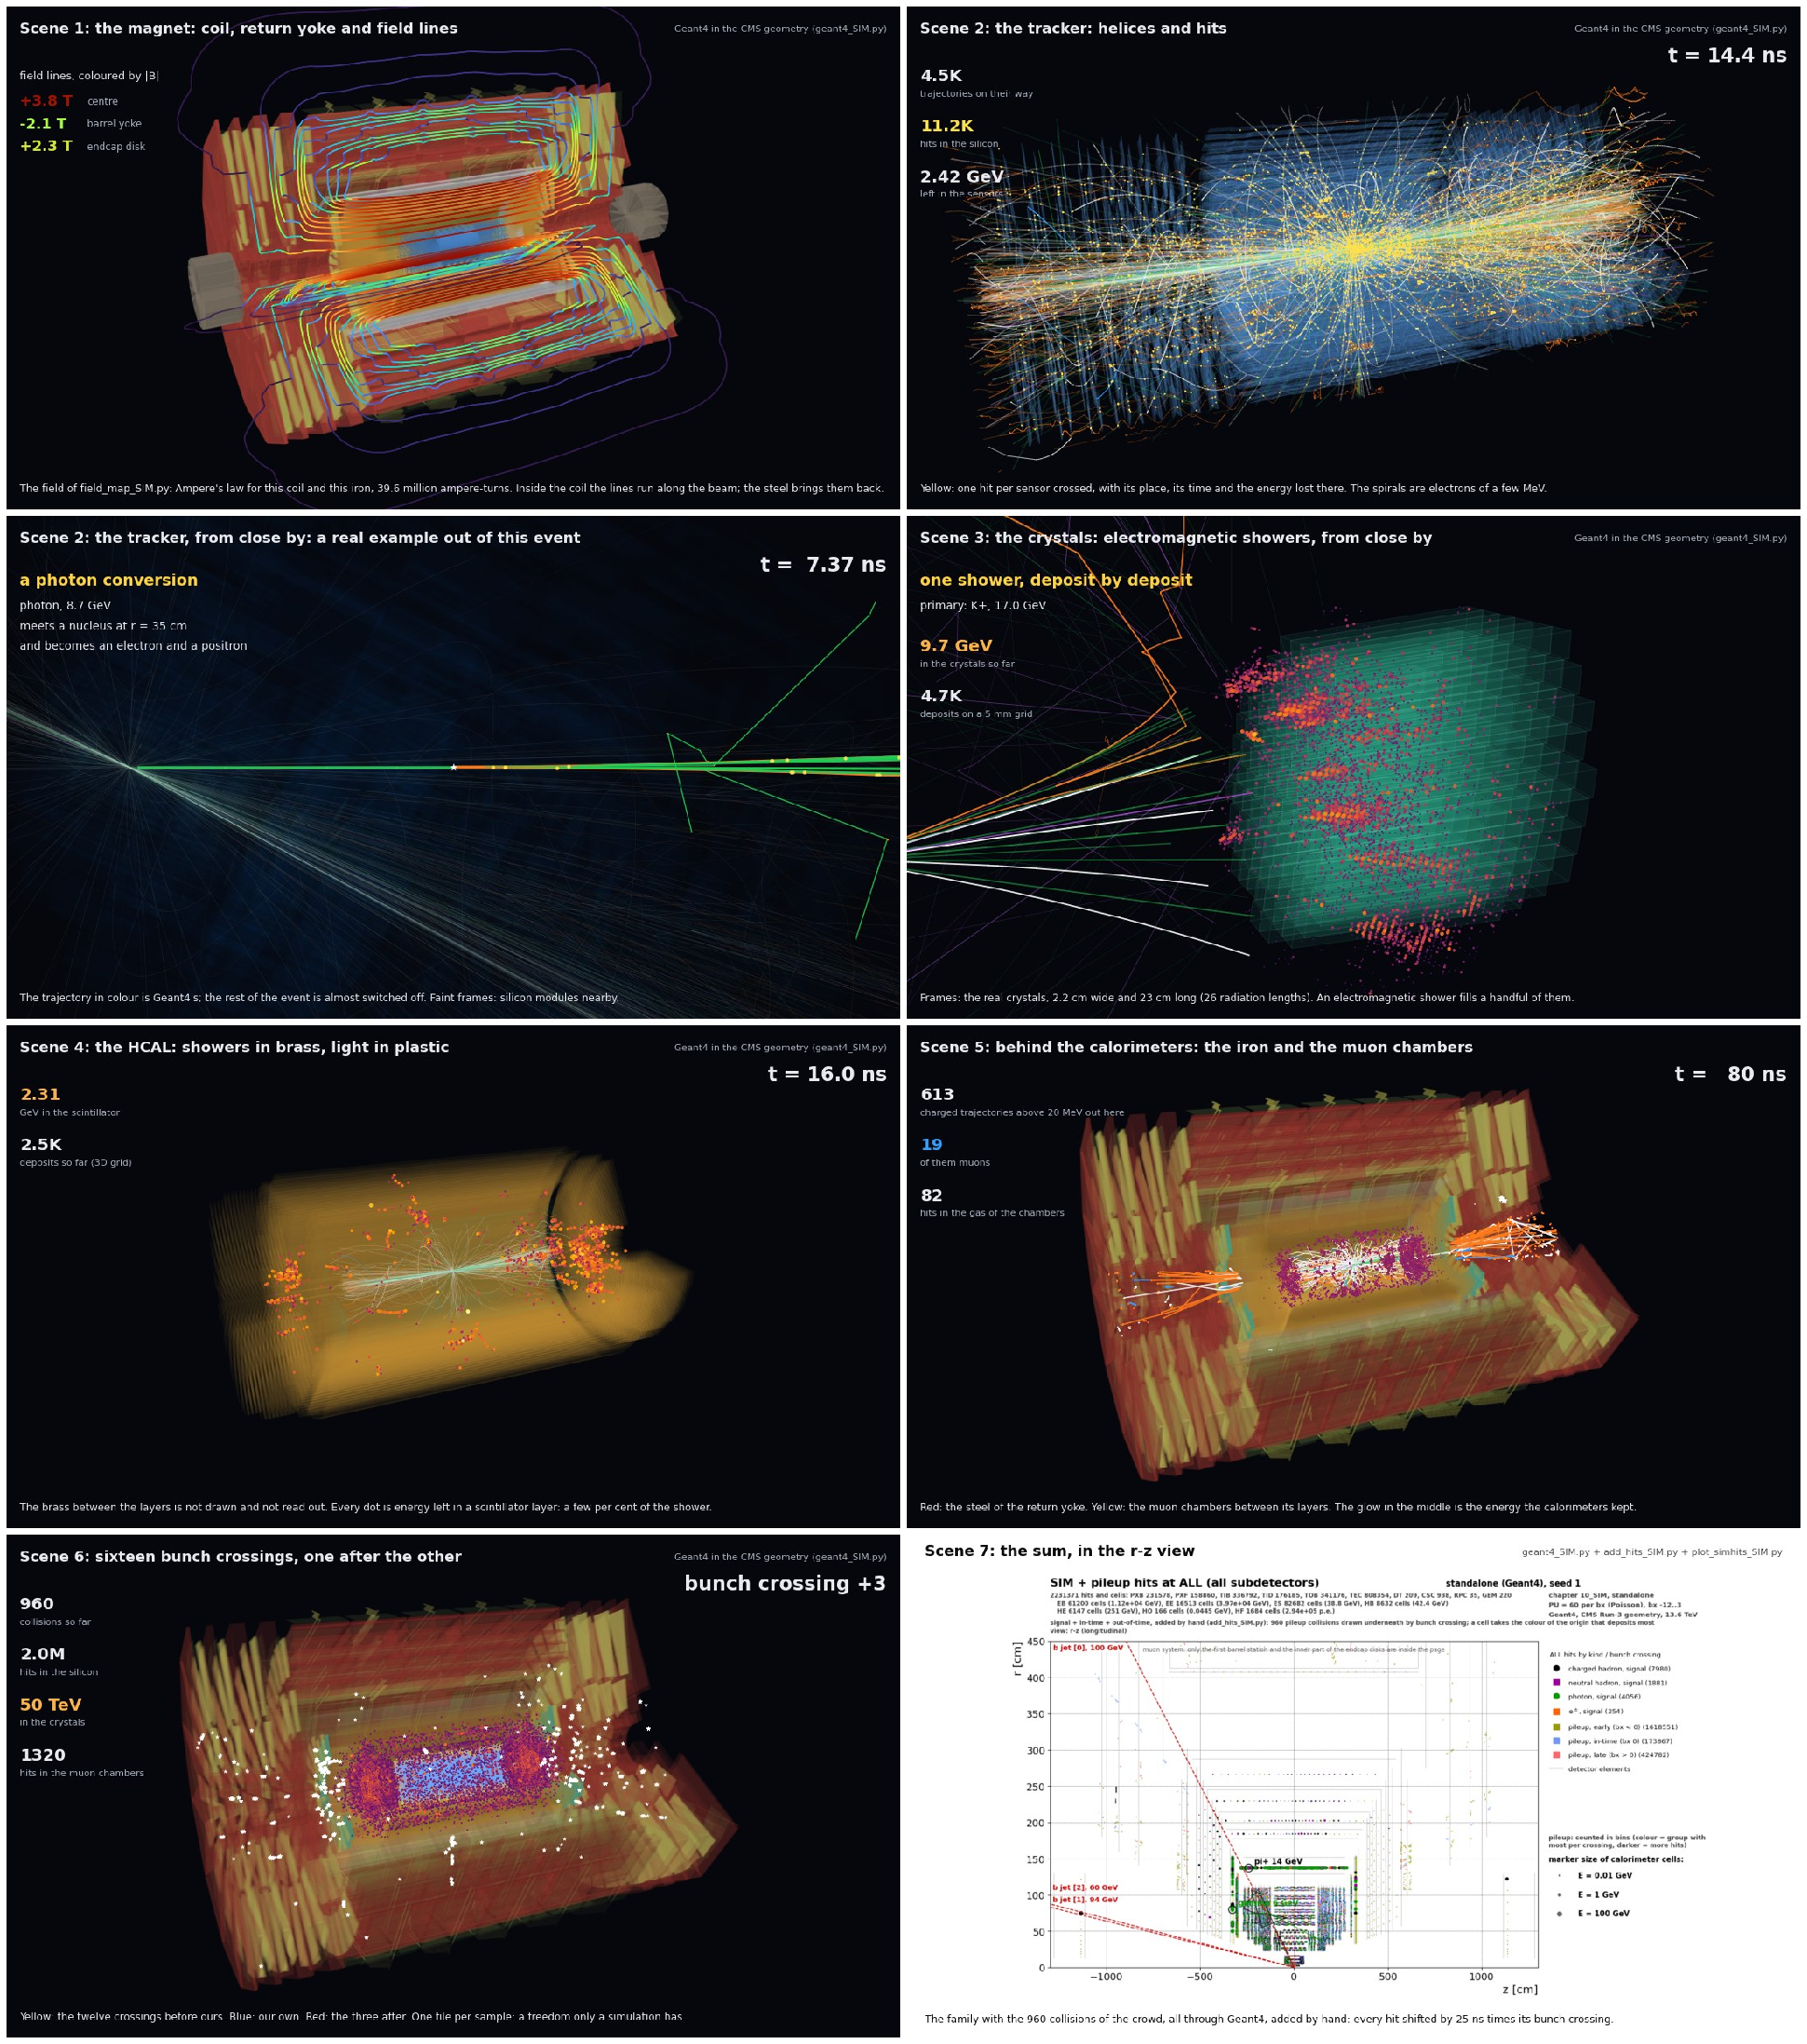
\includegraphics[width=\textwidth]{SIM/Standalone/animate_standalone_SIM_stills.pdf}
\caption[Key frames of the animated crossing]{Key frames of the animated
crossing (\file{animate_standalone_SIM.py}), $r$--$z$ view; dots are tracker
and muon hits, discs calorimeter cells. Top: the family $12\ns$ after the
collision (black), and the $63$ collisions of the same crossing (blue), each
sample simulated on its own. Bottom: the $897$ out-of-time collisions (olive
early, red late) on the clocks of their own crossings, and the sum on one
clock, $12\ns$ after our collision.}
\label{fig:crowd_at_the_border:stills}
\end{figure}

\paragraph{The picture to carry: one country, three crossings.}
\Cref{fig:crowd_at_the_border:chain} is the stop on one page. The same
detector and the same physics for everyone; three samples that never meet
inside the simulation; one addition at the end. The picture also says why
the production works this way: the crowd does not depend on the family, so
it can be simulated once and laid over any number of signal events.

\begin{figure}[htbp]\centering
\resizebox{0.9\textwidth}{!}{% chapter 10: the picture to carry. Three samples through the same detector, separately; their hits added by hand.
\begin{tikzpicture}[x=1cm,y=1cm,font=\footnotesize,>={Stealth[length=2mm]},
  box/.style={draw,rounded corners=2pt,minimum height=11mm,text width=2.55cm,align=center,inner sep=2pt},
  phys/.style={box,fill=black!6,text width=2.1cm},
  sig/.style={box,fill=red!12},it/.style={box,fill=blue!12},oot/.style={box,fill=olive!22},mx/.style={box,fill=orange!22}]
% the physics, switched on one after the other
\node[phys] (b) at (0,2.9)  {magnetic field\\{\scriptsize $R=p_T/0.3B$}};
\node[phys] (d) at (2.6,2.9) {decays in flight\\{\scriptsize $\beta\gamma c\tau$}};
\node[phys] (e) at (5.2,2.9) {EM physics\\{\scriptsize $X_0$}};
\node[phys] (h) at (7.8,2.9) {hadronic physics\\{\scriptsize $\lambda_I$}};
\draw[->] (b)--(d); \draw[->] (d)--(e); \draw[->] (e)--(h);
\draw[decorate,decoration={brace,amplitude=5pt,mirror}] (-1.2,2.2)--(9.0,2.2) node[midway,below=5pt]{the same detector and the same physics, in \GEANT, for every collision};
% three samples
\node[sig] (s)  at (-0.2,0.2)  {the family\\1 collision\\672 primaries};
\node[it]  (i)  at (3.9,0.2)  {in-time crowd\\63 collisions, bx $=0$\\10\,825 primaries};
\node[oot] (o)  at (8.0,0.2)  {out-of-time crowd\\897 collisions, 15 bx\\128\,894 primaries};
\node[sig] (sh) at (-0.2,-1.9) {\simChainSignal};
\node[it]  (ih) at (3.9,-1.9) {\simChainIntime};
\node[oot] (oh) at (8.0,-1.9) {\simChainOot};
\foreach \a/\b in {s/sh,i/ih,o/oh} \draw[->] (\a)--(\b) node[midway,right,font=\scriptsize]{simulated alone};
\node[mx,text width=5.2cm] (m) at (3.9,-4.0) {added by hand: $t\to t+25\,\mathrm{ns}\times\mathrm{bx}$,\\energies summed cell by cell\\\simChainSum};
\draw[->] (sh.south) |- (m.west); \draw[->] (ih)--(m); \draw[->] (oh.south) |- (m.east);
\draw[->] (m.south)--++(0,-0.55) node[below,font=\scriptsize,text=black!60]{the electronics: chapter 11};
\end{tikzpicture}
}
\caption[The stop on one page: three samples, one addition]{The stop on one
page. Top: the four ingredients of the simulation, switched on one after the
other in \cref{sec:crowd_at_the_border:theory}. Middle: the three samples and
what the tracker and the ECAL crystals receive from each. Bottom: the
addition by hand.}
\label{fig:crowd_at_the_border:chain}
\label{fig:crowd_at_the_border:windows_sketch}
\end{figure}

\paragraph{The number, three ways.}
\label{sec:crowd_at_the_border:validation}
\Cref{tab:crowd_at_the_border:numbers} compares the stop three ways. The
official package for the \emph{detector} is the CMS geometry itself: its
\textsc{TGeo} dump, the file of \cref{ch:crossing_the_border}, carries every
volume with its material, and ROOT's navigator~\cite{Brun:2003TGeo} follows
straight lines through it. The one-page detector of the script agrees with
it in the material in front of the calorimeters, to $1\,\%$ on average and
$8\,\%$ point by point in pseudorapidity (the layer thicknesses were tuned to
this scan, so the agreement is a closure, not a prediction), and in the
number of sensors a charged particle crosses, which was not tuned. For the
\emph{physics} the reference is the \CMSSW companion, which runs \GEANT
with the production list \code{FTFP\_BERT\_EMM} on its own event of the
same process. The two events are different draws, so the rows are compared
per primary or per collision; they agree to the tens of per cent a
parametrised simulation can claim, with one systematic difference: \GEANT
makes about $40\,\%$ more tracker hits per primary, the soft electrons and
nuclear fragments that the script does not create
(\cref{sec:crowd_at_the_border:caveats}). How each number is produced is in
the companion,
\begin{center}
  \companion{chapter_10_SIM}
\end{center}

\begin{table}[htbp]\centering\small
\caption[The crossing obtained three ways]{The crossing obtained three ways:
the standalone script (seed~1), the CMS simulation geometry scanned with
\textsc{TGeo}, and \GEANT in \CMSSW (run~1, event~1 of JitJetSW, another
event of the same process: $571$ primaries, $995$ pileup collisions).}
\label{tab:crowd_at_the_border:numbers}
\begin{tabular}{@{}lrrr@{}}\toprule
 & standalone & \textsc{TGeo} & \CMSSW 2025 \\ \midrule
material before the calorimeters, mean $x/\Xzero$ in $|\eta|<2.5$ & $1.16$ & $1.17$ & -- \\
\quad in interaction lengths, $x/\lamI$ & $0.33$ & $0.33$ & $\approx0.3$ \\
sensors crossed per charged primary, straight lines & $11.1$ & $11.8$ & $12.5$ \\
transverse momentum to reach the barrel ECAL [GeV] & $0.735$ & -- & $0.735$ \\ \midrule
tracker hits per primary, family, full physics & $12.8$ & -- & $18.0$ \\
energy loss per tracker hit [MeV] & $0.245$ & -- & $0.23$ \\
decays in flight per primary & $0.13$ & -- & $0.07$ \\
photons above $1\GeV$ that convert in the tracker & $40$ of $61$ & -- & $15$ of $29$ \\
charged hadrons that interact in the tracker & $34\,\%$ & -- & $26\,\%$ \\
HF photoelectrons, family & $1936$ & -- & $1849$ \\ \midrule
tracker hits per pileup collision & $1247$ & -- & $2107$ \\
ECAL energy per in-time collision [GeV] & $68$ & -- & $54$ \\
family's share of all tracker hits & $0.71\,\%$ & -- & $0.49\,\%$ \\
ECAL cells still dominated by the family & $1364$ of $7704$ & -- & $699$ of $12\,804$ \\
\bottomrule
\end{tabular}
\end{table}

\section{Let us dive into the details: the theory}
\label{sec:crowd_at_the_border:theory}

\subsection{The wind: the magnetic field}
\label{sec:crowd_at_the_border:field}
Why does a detector need a field? Because a tracker measures positions,
and only a curved path turns positions into a momentum. The solenoid of CMS
fills the tracker and the calorimeters with $3.8$~T along the beam. A
particle of charge $\pm1$ keeps its momentum along the field and turns in
the transverse plane on a circle of radius
\begin{equation}
  R\,[\mathrm{m}] = \frac{\pt\,[\mathrm{GeV}]}{0.3\,B\,[\mathrm{T}]}
  \quad\Rightarrow\quad R = 0.88~\mathrm{m}\times\pt\,[\mathrm{GeV}]\ \text{at}\ 3.8~\mathrm{T},
  \label{eq:crowd_at_the_border:radius}
\end{equation}
a helix in space (\cref{fig:crowd_at_the_border:helix_sketch}). A track from
the beam line gets no further from it than the diameter, so it reaches a
radius $r$ only if
\begin{equation}
  \pt > 0.3\,B\,r/2 ,
  \label{eq:crowd_at_the_border:looper}
\end{equation}
which is $0.735\GeV$ for the front face of the barrel ECAL at
$r=1.29$~m. Below it the particle is a \emph{looper}: it circles around the
beam, drifts along it and leaves the tracker through an end. A stiff track
is only deflected: its azimuth has turned by $\sin\Delta\phi=r/2R$ at radius
$r$, and over a chord $L$ it departs from the straight line by the sagitta
$s=L^2/8R$, the quantity the tracker measures.

\begin{figure}[htbp]\centering
\resizebox{0.88\textwidth}{!}{% chapter 10: the helix in the transverse plane, the sagitta and the looper.
\begin{tikzpicture}[x=1cm,y=1cm,font=\footnotesize,>={Stealth[length=2mm]}]
% (a) the circle and the sagitta
\begin{scope}
\node[font=\small\bfseries] at (2.2,4.15) {(a) a stiff track};
\draw[black!35] (0,0) circle (0.25); \draw[black!35] (0,0) ++(-10:3.3) arc (-10:75:3.3) node[above,black!60]{calorimeter, $r$};
\fill (0,0) circle (1.4pt) node[below left]{beam};
% circle of radius 6 through the origin, centre at (0,-6) rotated
\draw[red!80!black,thick] (0,0) arc (120:86.5:6.2);
\draw[dashed] (0,0)--(3.19,0.93) node[pos=0.62,below,sloped]{chord $L$};
\draw[<->] (1.6,0.47)--(1.47,0.92);
\draw[black!50,line width=0.3pt] (1.5,0.72)--(0.95,1.5) node[above,black]{sagitta $s=L^2/8R$};
\draw[->,black!60] (0,0)--(0.78,0.45) node[above left=-2pt,black!60]{$\vec p_T$};
\node[align=left] at (2.3,-1.25) {$R\,[\mathrm{m}]=\dfrac{p_T\,[\mathrm{GeV}]}{0.3\,B\,[\mathrm{T}]}$\\[2pt]$\sin\Delta\phi=r/2R$};
\node at (1.0,2.55) {$\odot\ \vec B$, 3.8 T};
\end{scope}
% (b) the looper
\begin{scope}[xshift=7.3cm]
\node[font=\small\bfseries] at (1.4,4.15) {(b) a looper};
\foreach \r in {0.5,1.0,1.5,2.0} \draw[black!25] (0,0) circle (\r);
\draw[black!35] (0,0) circle (3.0); \node[black!60] at (2.5,2.3) {$r$};
\fill (0,0) circle (1.4pt);
\draw[blue!70!black,thick] (0,-1.1) circle (1.1);
\draw[<->] (0,0)--(0,-2.2); \node at (0,-2.5) {$2R<r$};
\node[align=left] at (4.6,0.8) {never reaches $r$ if\\[2pt]$p_T<0.3\,B\,r/2$\\[2pt]$=0.735$~GeV\\for $r=1.29$~m};
\node[align=left] at (4.6,-1.4) {it crosses the\\same layers\\on every turn};
\end{scope}
\end{tikzpicture}
}
\caption[The helix in the transverse plane]{The helix in the transverse
plane. (a) A stiff track: radius, sagitta and the turn of the azimuth. (b) A
looper never reaches the calorimeter and crosses the same layers on every
turn.}
\label{fig:crowd_at_the_border:helix_sketch}
\end{figure}

For our event the log says: $307$ of the $672$ primaries are charged, $175$
of them inside the tracker, $|\eta|<2.5$, with a median \pt of $0.55\GeV$,
and $113$ of those are below $0.735\GeV$. Two thirds of the charged
particles a tracker sees can never reach the barrel calorimeter
(\cref{fig:crowd_at_the_border:field}). Switching the field on raises the
sensor crossings of the family from $3419$ on straight lines to $3830$ on
helices: the loopers cross the same layers again. The leading charged member
of our jet, a $\pi^+$ of $\pt=14.27\GeV$, has $R=12.5$~m; over $1.1$~m its
sagitta is $1.2\cm$ and its azimuth turns by $0.044$~rad. The jet as a
whole arrives at the calorimeters with $94.4$ instead of $99.8\GeV$ of
vector \pt: thirty-one tracks that no longer point where they were aimed.

\begin{figure}[htbp]\centering
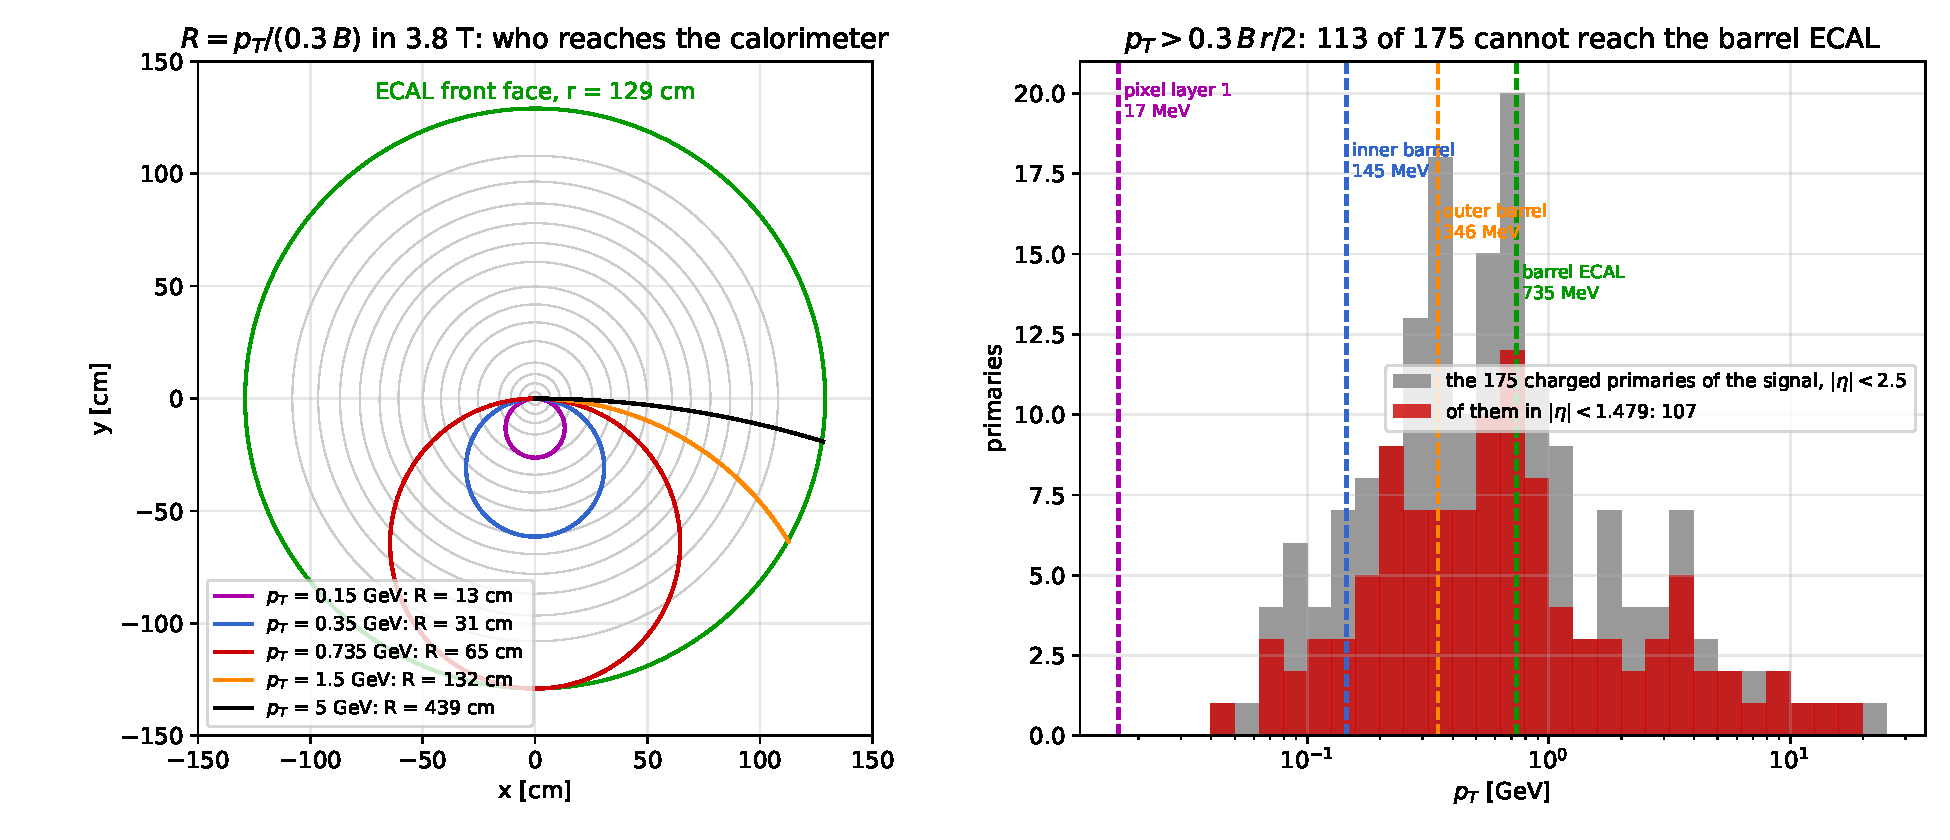
\includegraphics[page=1,width=\textwidth]{SIM/Standalone/theory_SIM.pdf}
\caption[The helix: who reaches the calorimeter]{\Cref{eq:crowd_at_the_border:radius,eq:crowd_at_the_border:looper}
for our event. Left: circles of positive particles from the beam line in
$3.8$~T, over the layers of the tracker; the red one, $0.735\GeV$, just
touches the ECAL. Right: the \pt of the charged primaries of the family and
the thresholds to reach the first pixel layer, the inner and the outer
barrel and the ECAL.}
\label{fig:crowd_at_the_border:field}
\end{figure}

\subsection{Dying on the way: decays in flight}
\label{sec:crowd_at_the_border:decays}
The generator decayed every hadron with $c\tau<10$~mm
(\cref{ch:crossing_the_border}); the long-lived ones were handed over
alive, and some of them die inside the detector. A particle of mass $m$ and
momentum $p$ flies on average $\beta\gamma c\tau=(p/m)\,c\tau$, and the
probability that it decays within a path $L$ is
\begin{equation}
  P(L) = 1-\exp\!\Big(-\frac{L\,m}{p\,c\tau}\Big).
  \label{eq:crowd_at_the_border:decay}
\end{equation}
The proper decay lengths make two classes
(\cref{fig:crowd_at_the_border:decay_sketch}): the $K^0_S$ ($d\bar s$ and
$s\bar d$, $c\tau=2.7\cm$) and the $\Lambda$ ($uds$, $7.9\cm$) decay inside
the tracker at a few \GeV, a displaced vertex of two tracks; the $\pi^\pm$
($7.8$~m) and $K^\pm$ ($3.7$~m) mostly reach the calorimeter, and when they
do decay they leave a muon and a neutrino that nobody sees.

\begin{figure}[htbp]\centering
\resizebox{0.92\textwidth}{!}{% chapter 10: who decays where. Mean flight beta gamma c tau on a scale of the detector.
\begin{tikzpicture}[x=0.085cm,y=1cm,font=\footnotesize,>={Stealth[length=2mm]}]
% the detector along a radius, in cm (0..160)
\fill[black!8] (2.25,-0.25) rectangle (16,2.95); \node[rotate=90,black!60] at (9,1.35) {pixel};
\fill[black!14] (22,-0.25) rectangle (110,2.95); \node[black!60] at (66,2.75) {strip tracker};
\fill[green!18] (129,-0.25) rectangle (152,2.95); \node[rotate=90,green!40!black] at (140.5,1.35) {ECAL crystals};
\draw[->] (0,-0.25)--(165,-0.25) node[right]{$r$ [cm]};
\foreach \x in {0,25,50,75,100,125,150} \draw (\x,-0.25)--(\x,-0.35) node[below]{\x};
% mean flights at p = 5 GeV
\draw[->,very thick,red!80!black] (0,2.3)--(27,2.3) node[right]{$K^0_S$, 5 GeV: $\beta\gamma c\tau=27$ cm $\to\pi^+\pi^-$ (a displaced vertex)};
\draw[->,very thick,violet] (0,1.6)--(35,1.6) node[right]{$\Lambda$, 5 GeV: 35 cm $\to p\,\pi^-$};
\draw[->,very thick,blue!70!black] (0,0.9)--(160,0.9); \node[blue!70!black,fill=white,inner sep=1pt] at (80,0.9) {$K^\pm$, 5 GeV: 38 m: 3\,\% decay before the ECAL};
\draw[->,very thick] (0,0.2)--(160,0.2); \node[fill=white,inner sep=1pt] at (80,0.2) {$\pi^\pm$, 5 GeV: 280 m: 0.5\,\% decay, $\pi\to\mu\nu$};
\end{tikzpicture}
}
\caption[Who decays where]{Who decays where: the mean flight
$\beta\gamma c\tau$ at $p=5\GeV$ on the radial scale of the detector.}
\label{fig:crowd_at_the_border:decay_sketch}
\end{figure}

The script draws the flight path of every such particle when it is born, as
$\beta\gamma c\tau\,(-\ln u)$ with $u$ uniform, and lets it decay there if
nothing else happens first, with the branching ratios of the table of
\cref{ch:children_producing_grandchildren}. In the full simulation of the
family $87$ particles decay in flight: $23$ $K^0_S$, $7$ $\Lambda$, $6$
$\Sigma^+$, one $K^0_L$, and $43$ pions and $7$ kaons, most of them
loopers, whose path of tens of metres makes up for their long lifetime
(\cref{fig:crowd_at_the_border:decay}). $48$ neutrinos leave unseen. The
fourth-hardest member of our jet, a $K^0_S$ of $18.7\GeV$, is one of them;
its two pions leave $102$ tracker hits that point back to no collision.

\begin{figure}[htbp]\centering
\includegraphics[page=2,width=\textwidth]{SIM/Standalone/theory_SIM.pdf}
\caption[Decays in flight]{\Cref{eq:crowd_at_the_border:decay}. Left: the
probability to decay within $1.23$~m of straight flight. Right: the $87$
decays in flight of the family in the $r$--$z$ plane of the tracker, the
$K^0_S$ and $\Lambda$ close to the beam, the looping pions everywhere.}
\label{fig:crowd_at_the_border:decay}
\end{figure}

\subsection{Footprints and tolls: electromagnetic physics in the tracker}
\label{sec:crowd_at_the_border:em}
\label{sec:crowd_at_the_border:every_collision}
A tracker should see a particle without disturbing it, and cannot: to be
seen the particle must lose energy in the sensor, and the sensor needs
supports, cables and cooling. Three things happen in every layer
(\cref{fig:crowd_at_the_border:em_sketch}a). A charged particle
\emph{ionises}: its mean energy loss per unit of matter is the Bethe-Bloch
formula~\cite{ParticleDataGroup:2024cfk},
\begin{equation}
  \Big\langle-\frac{dE}{dx}\Big\rangle = K\frac{Z}{A}\frac{1}{\beta^2}
  \Big[\tfrac12\ln\frac{2m_ec^2\beta^2\gamma^2T_{\max}}{I^2}-\beta^2-\frac{\delta}{2}\Big],
  \label{eq:crowd_at_the_border:bethe}
\end{equation}
a function of $\beta\gamma=p/m$ alone, with a minimum of $1.67\MeV\,\mathrm{cm^2/g}$
in silicon at $\beta\gamma\approx3.5$; in a thin sensor the loss fluctuates
with the long tail of Landau~\cite{Landau:1944if,Bichsel:1988if}, most
probably $84\keV$ and on average $124\keV$ in $320\um$. It is
\emph{scattered} by the nuclei, by an angle of width~\cite{Highland:1975pq,Lynch:1990sq}
\begin{equation}
  \theta_0=\frac{13.6\MeV}{\beta p}\sqrt{t}\,\big(1+0.038\ln t\big),\qquad t=x/\Xzero ,
  \label{eq:crowd_at_the_border:highland}
\end{equation}
$1.9$~mrad for a pion of $1\GeV$ crossing a layer of $2.5\,\%$ of a
radiation length. And the two lightest travellers pay a toll measured in the
same unit, the radiation length \Xzero~\cite{Tsai:1973py}: an electron
radiates, keeping on average $e^{-t}$ of its energy, and a photon converts
into an $e^+e^-$ pair with the probability
\begin{equation}
  P_{\mathrm{conv}}=1-e^{-7t/9}.
  \label{eq:crowd_at_the_border:conversion}
\end{equation}

\begin{figure}[htbp]\centering
\resizebox{\textwidth}{!}{% chapter 10: electromagnetic physics. What a layer of material does, and the shower in a crystal.
\begin{tikzpicture}[x=1cm,y=1cm,font=\footnotesize,>={Stealth[length=2mm]}]
% (a) a layer of the tracker
\node[font=\small\bfseries] at (2.3,3.3) {(a) one layer of silicon and its support};
\fill[black!15] (2.0,-0.3) rectangle (2.5,2.9); \node[rotate=90] at (2.25,1.3) {$t=x/X_0$};
% charged hadron
\draw[thick] (0,2.5)--(2.25,2.5); \draw[thick,->] (2.25,2.5)--(4.6,2.75) node[right]{$\pi$: loses $dE/dx$, scattered by $\theta_0$};
\fill[red] (2.25,2.5) circle (2pt) node[above left,red!70!black]{hit};
% electron
\draw[thick,orange!90!black] (0,1.5)--(2.25,1.5); \draw[thick,orange!90!black,->] (2.25,1.5) to[bend right=12] (4.6,1.05) node[right]{$e$: bremsstrahlung};
\draw[decorate,decoration={snake,amplitude=1pt,segment length=4pt},green!50!black,->] (2.25,1.5)--(4.6,1.62) node[right]{$\gamma$};
\fill[red] (2.25,1.5) circle (2pt);
% photon
\draw[decorate,decoration={snake,amplitude=1pt,segment length=4pt},green!50!black] (0,0.4)--(2.25,0.4);
\draw[thick,orange!90!black,->] (2.25,0.4) to[bend left=10] (4.6,0.85) node[right]{$e^+$};
\draw[thick,orange!90!black,->] (2.25,0.4) to[bend right=10] (4.6,-0.05) node[right]{$e^-$\quad conversion, $P=1-e^{-7t/9}$};
% (b) the shower in a crystal
\begin{scope}[xshift=9.6cm,yshift=1.3cm]
\node[font=\small\bfseries] at (2.4,2.0) {(b) the shower in a crystal};
\draw[fill=green!10] (0,-0.55) rectangle (5.0,0.55); \draw[black!40] (0,-1.65) rectangle (5.0,-0.55); \draw[black!40] (0,0.55) rectangle (5.0,1.65);
\draw[decorate,decoration={snake,amplitude=1pt,segment length=4pt},green!50!black,->] (-1.2,0)--(0.5,0);
\foreach \a in {-22,-12,-4,4,12,22} \draw[orange!90!black] (0.5,0)--++(\a:1.5);
\foreach \a in {-30,-20,-10,0,10,20,30} \draw[orange!90!black!70] (1.9,0.0)++(0,{\a/60})--++(\a:1.1);
\draw[<->] (0,-1.9)--(5.0,-1.9) node[midway,below]{23 cm $=25.8\,X_0$};
\draw[<->] (5.25,-0.55)--(5.25,0.55) node[midway,right]{2.2 cm $=1\,R_M$};
\draw[->] (1.75,1.95)--(1.75,0.6); \node[above] at (1.75,1.95) {$t_{max}\approx\ln(E/E_c)$};
\end{scope}
\end{tikzpicture}
}
\caption[Electromagnetic physics in a layer and in a crystal]{(a) What one
layer of the tracker does to a pion, an electron and a photon. (b) The
electromagnetic shower in a crystal of the ECAL
(\cref{sec:crowd_at_the_border:shower}).}
\label{fig:crowd_at_the_border:em_sketch}
\end{figure}

How many radiation lengths? \Cref{fig:crowd_at_the_border:material} is the
answer of the CMS geometry: $0.34\,\Xzero$ at $\eta=0$, rising to $2.0$ at
$|\eta|=1.4$, where the cables and pipes of the barrel leave the tracker,
and about $1.3$ beyond; in interaction lengths, the unit of
\cref{sec:crowd_at_the_border:hadronic}, $0.13$ to $0.45$. The script
reproduces the curve with $54$ surfaces. The consequence is on the right of
the figure: more than half of the photons convert before they reach the
calorimeter.

\begin{figure}[htbp]\centering
\includegraphics[page=4,width=\textwidth]{SIM/Standalone/theory_SIM.pdf}
\caption[The material of the tracker and what it does]{Left: the material
between the beam and the calorimeters in radiation lengths and in
interaction lengths, in the CMS simulation geometry (solid, \textsc{TGeo};
band: spread over azimuth) and in the layer model of the script (dashed).
Right: \cref{eq:crowd_at_the_border:conversion} and its hadronic twin
evaluated with the CMS material (lines), and the fraction of $5\GeV$ photons
and pions lost in the script before the calorimeters (points): $57\,\%$ and
$28\,\%$ on average.}
\label{fig:crowd_at_the_border:material}
\end{figure}

With electromagnetic physics on, the family's tracker hits carry an energy
loss, $2.10\GeV$ in $8585$ hits of the full simulation, $0.245\MeV$ per hit
(median $128\keV$; \cref{fig:crowd_at_the_border:bethe}). $313$ photons
convert, half of them in the services at the ends of the barrels, and the
electrons radiate $676$ photons above $10\MeV$. Of the $61$ primary photons
above $1\GeV$ inside the tracker, $40$ convert: by
\cref{eq:crowd_at_the_border:conversion} they crossed $1.4\,\Xzero$ on
average, as most of them fly towards the endcaps. $469$ particles, soft
electrons and loopers, stop in the tracker and never reach a calorimeter.

\begin{figure}[htbp]\centering
\includegraphics[page=3,width=\textwidth]{SIM/Standalone/theory_SIM.pdf}
\caption[The energy loss in silicon]{\Cref{eq:crowd_at_the_border:bethe}.
Left: the mean energy loss in silicon against $\beta\gamma$. Right: the
energy lost in the sensor by the family's hits in three subdetectors: a
Landau peak, shifted by the thickness and by the angle of incidence, and a
tail of slow particles.}
\label{fig:crowd_at_the_border:bethe}
\end{figure}

\subsection{The wall of crystal: the electromagnetic shower}
\label{sec:crowd_at_the_border:shower}
What stops a photon of $40\GeV$ in $23\cm$? Its own multiplication. In
lead tungstate, $\Xzero=0.89\cm$, a photon converts and an electron radiates
every centimetre, so the number of particles doubles and their energy
halves until it reaches the critical energy $E_c\approx9\MeV$, where
ionisation wins (\cref{fig:crowd_at_the_border:em_sketch}b). The energy
deposited per radiation length follows a Gamma
distribution~\cite{Grindhammer:1993kw},
\begin{equation}
  \frac{1}{E}\frac{dE}{dt}=\frac{\beta\,(\beta t)^{\alpha-1}e^{-\beta t}}{\Gamma(\alpha)},
  \qquad t_{\max}=\frac{\alpha-1}{\beta}\approx\ln\frac{E}{E_c}-0.8 ,
  \label{eq:crowd_at_the_border:gamma}
\end{equation}
with a maximum that moves only logarithmically with the energy: $3.9$,
$6.2$ and $8.5\,\Xzero$ at $1$, $10$ and $100\GeV$. A crystal of $25.8\,\Xzero$
contains them all. Across, the scale is the Moli\`ere radius, $2.19\cm$ in
lead tungstate and the width of a barrel crystal: $90\,\%$ of the energy
falls within one. The script draws $\alpha$ and $t_{\max}$ with their
fluctuations and correlation for every shower, places up to $250$ spots of
equal energy by \cref{eq:crowd_at_the_border:gamma} and a two-component
radial profile, and adds each spot to the crystal it falls in.

\Cref{fig:crowd_at_the_border:shower} shows what the tracker in front does
to this picture. Of $400$ photons of $10\GeV$ at $\eta=0.5$, the $263$
that arrive unconverted put $71\,\%$ of their energy into one crystal and
$90\,\%$ into four. The $137$ that converted arrive as two or more particles
bent apart by the field: $44\,\%$ in the hottest crystal, $90\,\%$ in ten.
Same photon, same calorimeter. The family leaves $206\GeV$ in $2984$ barrel
crystals and $411\GeV$ in $2937$ endcap crystals.

\begin{figure}[htbp]\centering
\includegraphics[page=6,width=\textwidth]{SIM/Standalone/theory_SIM.pdf}
\caption[The electromagnetic shower]{\Cref{eq:crowd_at_the_border:gamma}.
Left: the mean longitudinal profile in lead tungstate for three energies.
Right: the share of the hottest, the $9$ and the $25$ hottest crystals for
photons of $10\GeV$, unconverted (green) and converted in the tracker
(orange); bars are the spread from photon to photon.}
\label{fig:crowd_at_the_border:shower}
\end{figure}

\subsection{The wall of brass: hadronic physics}
\label{sec:crowd_at_the_border:hadronic}
\label{sec:crowd_at_the_border:in_out_of_time}
A hadron also meets the nuclei through the strong force, and its unit of
length is the nuclear interaction length \lamI, the mean path before an
inelastic collision: $20\cm$ in lead tungstate, twenty times the radiation
length. After a thickness $x$ a fraction
\begin{equation}
  P_{\mathrm{int}}=1-e^{-x/\lamI}
  \label{eq:crowd_at_the_border:lambda}
\end{equation}
has interacted. Three consequences follow. In the tracker, $0.3\,\lamI$ on
average, a third of the hadrons break up before any calorimeter: in our
event $163$ nuclear interactions, and $32$ of the $93$ charged hadrons above
$0.5\GeV$, $34\,\%$. In the crystals, $1.13\,\lamI$ deep, two hadrons in
three start their shower already in the ECAL, and one in three crosses it
as a minimum-ionising particle leaving a quarter of a \GeV. And the shower
itself is not like a photon's
(\cref{fig:crowd_at_the_border:had_sketch})~\cite{Wigmans:2000vf,Fabjan:2003aq}.
The $\pi^0$ made in every interaction decay at once to photons, and that
part of the energy showers electromagnetically; its mean fraction grows
slowly with the energy~\cite{Gabriel:1993ai,Groom:2006am},
\begin{equation}
  f_{em}=1-\Big(\frac{E}{E_0}\Big)^{k-1},\qquad E_0\approx0.8\GeV\ (\pi),\quad k\approx0.82 ,
  \label{eq:crowd_at_the_border:fem}
\end{equation}
$0.37$ at $10\GeV$ and $0.58$ at $100\GeV$, and fluctuates from one shower
to the next. Of the rest a part is \emph{invisible}: it breaks nuclei, or
leaves as slow neutrons and neutrinos. A calorimeter therefore sees a
hadron as $f_{em}+(1-f_{em})\,h/e$ of an electron of the same energy, with
$h/e\approx0.6$ to $0.7$. Finally the HCAL is a \emph{sampling}
calorimeter: brass plates stop the shower and only the thin scintillator
tiles between them are sensitive, about $1\,\%$ of the energy. A calorimeter
hit of the HCAL is that $1\,\%$; the digitisation of
\cref{ch:customs_form} multiplies it back.

\begin{figure}[htbp]\centering
\resizebox{\textwidth}{!}{% chapter 10: the hadronic shower in ECAL + HCAL: where the energy of a pion goes.
\begin{tikzpicture}[x=1cm,y=1cm,font=\footnotesize,>={Stealth[length=2mm]}]
\fill[green!12] (0,-1.5) rectangle (1.3,1.5); \node[above,align=center] at (0.65,1.5) {crystals\\$1.1\,\lambda_I$};
\foreach \x in {2.2,2.9,3.6,4.3,5.0,5.7,6.4,7.1} {\fill[orange!35] (\x,-1.5) rectangle (\x+0.5,1.5); \fill[blue!35] (\x+0.5,-1.5) rectangle (\x+0.7,1.5);}
\node[above,align=center] at (5.0,1.5) {HCAL: brass and scintillator\\$5.6\,\lambda_I$ at $\eta=0$};
\draw[thick,->] (-1.4,0)--(0,0); \node[above] at (-0.9,0.05) {$\pi^+$};
\draw[thick,dashed] (0,0)--(2.9,0); \node[below,font=\scriptsize] at (0.65,-0.1) {ionises};
\fill (2.9,0) circle (2pt);
\foreach \a/\l in {28/1.9,14/2.8,-8/3.2,-24/2.2} \draw[thick] (2.9,0)--++(\a:\l);
\draw[decorate,decoration={snake,amplitude=1pt,segment length=4pt},green!50!black,thick] (2.9,0)--++(5:1.3) node[right,font=\scriptsize]{$\pi^0\to\gamma\gamma$};
\draw[dotted,thick] (2.9,0)--++(55:1.6) node[above,font=\scriptsize]{$n$};
\draw[dotted,thick] (2.9,0)--++(-60:1.5) node[below,font=\scriptsize]{$n$};
% the budget
\begin{scope}[xshift=9.2cm,yshift=1.1cm]
\node[anchor=west,font=\small\bfseries] at (0,0.75) {a pion of $E$};
\draw[fill=green!30] (0,0) rectangle (2.2,0.5) node[midway]{$f_{em}E$};
\draw[fill=orange!30] (2.2,0) rectangle (4.6,0.5) node[midway]{charged hadrons};
\draw[fill=black!20] (4.6,0) rectangle (6.0,0.5) node[midway]{invisible};
\node[anchor=west,align=left] at (0,-0.75) {$f_{em}=1-(E/E_0)^{k-1}$: 0.37 at 10 GeV, 0.58 at 100 GeV};
\node[anchor=west,align=left] at (0,-1.45) {invisible: nuclear binding, slow neutrons, neutrinos};
\node[anchor=west,align=left] at (0,-2.15) {seen: $f_{em}+(1-f_{em})\,h/e$, and of that only the};
\node[anchor=west,align=left] at (0,-2.65) {scintillator's share, below 1\,\% (the sampling fraction)};
\end{scope}
\end{tikzpicture}
}
\caption[The hadronic shower]{A pion in the calorimeters: it ionises until
its first inelastic interaction, and the shower is part electromagnetic,
part hadronic, part invisible.}
\label{fig:crowd_at_the_border:had_sketch}
\end{figure}

The script draws the depth of the first interaction from
\cref{eq:crowd_at_the_border:lambda}, the electromagnetic fraction from
\cref{eq:crowd_at_the_border:fem} with its fluctuation, and places the
hadronic part with the longitudinal profile of Bock et
al.~\cite{Bock:1980rs} in interaction lengths. For the family, $221$ hadrons
start their shower in the crystals and $78$ in the HCAL; $158\GeV$ are
invisible, $124\GeV$ fall into the dead material between and behind the
calorimeters, and the scintillator of the barrel and endcap HCAL holds
$2.5\GeV$. \Cref{fig:crowd_at_the_border:hadronic} sends single pions into
the barrel: crystals and scintillator together, the latter multiplied by its
sampling factor, give back $0.77$ of a pion of $2\GeV$ and $0.85$ of one of
$50\GeV$, with $41\,\%$ of it in the crystals. This is the non-linear
response the jet energy corrections of \cref{ch:fair_price} exist for, and
the test beams of CMS measured the same shape~\cite{USCMS:2009fxn}. The
forward calorimeter is a different instrument: quartz fibres in steel that
see only Cherenkov light, counted in photoelectrons; the family leaves
$1936$ of them.

\begin{figure}[htbp]\centering
\includegraphics[page=7,width=\textwidth]{SIM/Standalone/theory_SIM.pdf}
\caption[The hadronic shower: electromagnetic fraction and response]{\Cref{eq:crowd_at_the_border:fem}.
Left: the electromagnetic fraction for pions and protons, and what the HCAL
and the crystals see. Right: the response of crystals plus HCAL to single
pions in the script, the share of the crystals in it, and the fraction of
pions that cross the crystals without interacting, $e^{-1.13}=0.32$.}
\label{fig:crowd_at_the_border:hadronic}
\end{figure}

\subsection{Three crowds, one clock: the addition}
\label{sec:crowd_at_the_border:crossing_frame}
\label{sec:crowd_at_the_border:premixing}
\label{sec:crowd_at_the_border:truth}
Why simulate the crowd apart? Because nothing in the detector couples two
collisions: a hit is made by one particle in one piece of matter. The hits
of an event are therefore the plain sum of the hits of its collisions, and
the only thing the sum must respect is the clock
(\cref{fig:crowd_at_the_border:clock}). A collision of bunch crossing \bx
happens $25\ns\times\bx$ away from ours, so a hit it makes at time
$t_{\mathrm{flight}}$ after its own crossing appears at
\begin{equation}
  t=t_{\mathrm{flight}}+25\ns\times\bx,\qquad
  E_{\mathrm{cell}}=\sum_{\bx=-12}^{+3}\ \sum_{\mathrm{hits}\,\in\,\bx}E_{\mathrm{hit}} .
  \label{eq:crowd_at_the_border:sum}
\end{equation}
That is all \file{add_hits_SIM.py} does, and all the \Mix of \CMSSW does at
this level~\cite{Hildreth:2017caz}: it stamps every hit with its crossing
and its collision, and lays them in one frame.

\begin{figure}[htbp]\centering
\resizebox{0.95\textwidth}{!}{% chapter 10: sixteen bunch crossings on one clock, and one cell that adds them.
\begin{tikzpicture}[x=0.72cm,y=1cm,font=\footnotesize,>={Stealth[length=2mm]}]
\draw[->] (-13,0)--(5,0) node[right]{$t$};
\foreach \b/\n in {-12/60,-11/56,-10/68,-9/61,-8/66,-7/56,-6/55,-5/50,-4/53,-3/66,-2/61,-1/60} {
  \fill[olive!70] (\b-0.3,0) rectangle (\b+0.3,{\n/45}); \node[font=\tiny] at (\b,{\n/45+0.15}) {\n}; \node[font=\tiny,below] at (\b,0) {\b};}
\fill[blue!60] (-0.3,0) rectangle (0.3,{63/45}); \node[font=\tiny] at (0.15,{63/45+0.15}) {63};
\fill[red!80!black] (-0.3,{63/45}) rectangle (0.3,{63/45+0.25}); \node[font=\tiny,red!80!black,anchor=west] at (0.35,{63/45+0.32}) {+ the family};
\node[font=\tiny,below] at (0,0) {\textbf{0}};
\foreach \b/\n in {1/63,2/59,3/63} {\fill[red!45] (\b-0.3,0) rectangle (\b+0.3,{\n/45}); \node[font=\tiny] at (\b,{\n/45+0.15}) {\n}; \node[font=\tiny,below] at (\b,0) {+\b};}
\node[below] at (-12,-0.3) {$-300$ ns}; \node[below] at (0,-0.3) {0}; \node[below] at (3,-0.3) {$+75$ ns};
\draw[decorate,decoration={brace,amplitude=5pt}] (-12.3,2.0)--(-0.7,2.0) node[midway,above=5pt]{early: 712 collisions, simulated one by one};
\draw[decorate,decoration={brace,amplitude=5pt}] (0.7,2.0)--(3.3,2.0) node[midway,above=5pt]{late: 185};
% one cell
\node[draw,fill=green!12,minimum width=1.6cm,minimum height=1.1cm,align=center] (c) at (-4,-2.3) {one cell\\$E=\sum_{bx}\sum_{hits}E_{hit}$};
\foreach \b in {-10,-7,-3,0,2} \draw[->,black!60] (\b,-0.75) -- (c);
\node[align=left,anchor=west] at (-1.6,-2.3) {every hit keeps its time $t=t_{flight}+25\,\mathrm{ns}\times bx$\\and the collision it came from; nothing is lost in the sum};
\end{tikzpicture}
}
\caption[Sixteen crossings on one clock]{Sixteen bunch crossings on one
clock: the collisions drawn for each in \cref{ch:crowd_on_the_road}, and one
cell that adds what all of them leave in it.}
\label{fig:crowd_at_the_border:clock}
\end{figure}

The crowd is very unequal. A collision leaves $8.6$ tracker hits per
primary and $1247$ on average, but the median is $725$ and the largest
leaves $8102$; in the crystals $57\GeV$ on average. On one clock
(\cref{fig:crowd_at_the_border:time}) the sixteen crossings are sixteen
bursts of hits $25\ns$ apart, each with a tail of loopers and slow
particles that reaches into the next; the family's $8585$ hits are one line
under the burst of the $92\,942$ of its own crossing. In the circle of our
jet, $\Delta R<0.4$, the cells receive $66\GeV$ of transverse energy from
the family and $231\GeV$ from the crowd, $14.5\GeV$ per crossing and
$15.5\GeV$ from our own. Which of the fifteen other crossings a detector
still sees is decided by its electronics: the tracker listens for one
crossing, the crystals and the tiles for several. That is
\cref{ch:customs_form}; here every hit is kept, with its time.

\begin{figure}[htbp]\centering
\includegraphics[page=8,width=\textwidth]{SIM/Standalone/theory_SIM.pdf}
\caption[The three crowds in time]{\Cref{eq:crowd_at_the_border:sum}. Left:
the time of every tracker hit after the shift, by origin. Right: the
transverse energy the cells within $\Delta R<0.4$ of our jet receive from
each bunch crossing (HCAL cells multiplied by their sampling factor).}
\label{fig:crowd_at_the_border:time}
\end{figure}

\paragraph{The recipe.}
\Cref{fig:crowd_at_the_border:flow} is the loop the script runs for every
particle. (1)~Take a particle from the stack and, if it is unstable, draw
its decay path. (2)~Follow the helix, or the line, to the next surface of
the tracker. (3)~If the decay path ends first, decay and stack the
daughters. (4)~At the surface: record a hit if it is a sensor; subtract the
energy loss of \cref{eq:crowd_at_the_border:bethe}; scatter by
\cref{eq:crowd_at_the_border:highland}; let an electron radiate, a photon
convert by \cref{eq:crowd_at_the_border:conversion}, a hadron interact by
\cref{eq:crowd_at_the_border:lambda}, and stack what comes out. (5)~At the
boundary of the tracker follow the particle to the face of the ECAL or of
the HF. (6)~There a photon or electron showers by
\cref{eq:crowd_at_the_border:gamma}; a hadron ionises to its first
interaction and showers by \cref{eq:crowd_at_the_border:fem}; a muon ionises
through everything to the muon stations. (7)~Repeat for the $672$ primaries
of the family, then, with other random numbers, for each collision of the
crowd on the clock of its own crossing. (8)~Add by
\cref{eq:crowd_at_the_border:sum}.

\begin{figure}[htbp]\centering
\resizebox{\textwidth}{!}{% chapter 10: the recipe of standalone_SIM.py for one particle.
\begin{tikzpicture}[x=1cm,y=1cm,font=\footnotesize,>={Stealth[length=2mm]},
  b/.style={draw,rounded corners=2pt,fill=black!5,minimum height=9mm,text width=2.9cm,align=center,inner sep=2pt},
  d/.style={draw,diamond,aspect=2.4,fill=yellow!15,inner sep=1pt,align=center,text width=2.1cm}]
\node[b] (a) at (0,0) {take a particle from the stack; draw its decay path $\beta\gamma c\tau(-\ln u)$};
\node[b] (h) at (4.2,0) {helix (or line) to the next surface of the tracker};
\node[d] (q) at (8.5,0) {decay path reached first?};
\node[b] (dc) at (12.6,0) {decay: daughters on the stack};
\node[b] (m) at (8.5,-2.3) {at the surface: hit, $dE/dx$, scattering, bremsstrahlung, conversion, nuclear interaction};
\node[d] (e) at (4.2,-2.3) {boundary of the tracker?};
\node[b] (c) at (0,-2.3) {to the face of ECAL or HF; shower, or ionise through to the muon stations};
\node[b,fill=green!12] (o) at (0,-4.3) {cells: energy and time per primary};
\node[b,fill=red!10] (t) at (8.5,-4.3) {tracker hit: position, time, $dE$, primary};
\draw[->] (a)--(h); \draw[->] (h)--(q); \draw[->] (q)--node[above]{yes}(dc); \draw[->] (q)--node[right]{no}(m);
\draw[->] (m)--(e); \draw[->] (e)--node[above]{yes}(c); \draw[->] (e)--node[right]{no}(h);
\draw[->] (c)--(o); \draw[->] (m)--(t);
\draw[->] (dc.north) -- ++(0,0.5) -| (a.north);
\draw[->] (m.east) -- ++(1.0,0) node[right,align=left]{secondaries\\on the stack};
\end{tikzpicture}
}
\caption[The recipe of the standalone simulation]{The loop of
\file{standalone_SIM.py} for one particle.}
\label{fig:crowd_at_the_border:flow}
\end{figure}

\section{The energy ledger: our jet at this stage}
\label{sec:crowd_at_the_border:ledger}

The record \file{example/SIM/event_SIM.lhe} is the record of
\cref{ch:crossing_the_border} followed by three tables: the summary of the
hits, one row per primary of the family (what ended it as a primary, where
it left the tracker, its hits and the energy it left in each calorimeter),
and one row per collision of the crowd. The hits themselves, $1.2$ million
points and $200\,000$ cells, are in three binary files, one per sample.
\Cref{tab:crowd_at_the_border:stages} is the family alone, one ingredient
more in each row, and \cref{tab:crowd_at_the_border:hits_ledger} is the
ledger of the three samples and of their sum.

\begin{table}[htbp]\centering\scriptsize\setlength{\tabcolsep}{2.6pt}
\caption[The physics switched on stage by stage]{The physics switched on
stage by stage, for the family (\file{standalone_SIM.log}): primaries
leaving the tracker intact (of $672$), stored secondaries and their origin
(decay / electromagnetic / hadronic), tracker and muon-chamber hits, the
energy lost in the sensors [GeV], calorimeter cells, energy per subdetector
(GeV; HB, HE: in the scintillator; HF: photoelectrons), and our jet: vector
\pt [GeV] of its members still primaries at the boundary (their number) and
the energy they leave in the crystals. The $955$ muon-chamber hits of the
fourth row are hadrons crossing the calorimeters like muons, as long as
nothing makes them interact.}
\label{tab:crowd_at_the_border:stages}
\resizebox{\textwidth}{!}{%
\begin{tabular}{@{}lrrrrrrrrrrrrrr@{}}\toprule
stage & bound. & \multicolumn{2}{c}{secondaries} & \multicolumn{2}{c}{hits} & $\sum dE$ & cells & EB & EE & HB & HE & HF & jet \pt & jet \\
 & & all & dec/EM/had & tracker & muon & & & & & & & & at bound. & ECAL \\ \midrule
\simStageRows
\bottomrule
\end{tabular}}
\end{table}

\begin{table}[htbp]\centering\footnotesize\setlength{\tabcolsep}{4pt}
\caption[The ledger of the hits: three samples and their sum]{The ledger of
the hits (\file{add_hits_SIM.log}): the family, the in-time crowd and the
out-of-time crowd, split into its twelve early and three late crossings,
each simulated separately, and their sum. For cells the last column is the
number of distinct cells. Below the line every cell of the sum is given to
the origin that deposited most of its energy, as the \CMSSW companion's
ledger does.}
\label{tab:crowd_at_the_border:hits_ledger}
\begin{tabular}{@{}lrrrrr@{}}\toprule
 & the family & in time & early & late & added \\
 & & \bx $=0$ & \bx $-12\ldots-1$ & \bx $+1\ldots+3$ & \\ \midrule
\simLedgerRows
\bottomrule
\end{tabular}
\end{table}

\paragraph{Station by station.}
\label{sec:crowd_at_the_border:stations}
\Cref{tab:crowd_at_the_border:trk,tab:crowd_at_the_border:calo,tab:crowd_at_the_border:muon}
take the same sum detector by detector, and
\cref{fig:crowd_at_the_border:stations_signal,fig:crowd_at_the_border:stations_mixed}
draw it. In the \emph{tracker} the endcap disks of the strip tracker hold $41\,\%$ of the hits,
the family's and the crowd's alike, and the family is $8.5\,\%$ of the hits
of its own crossing and $0.7\,\%$ of all sixteen. In the \emph{ECAL} the
crowd reaches $99\,\%$ of the barrel crystals and every endcap crystal; the
family deposits in $7704$ cells and remains the largest depositor in $1364$
of them, which hold $428$ of its $617\GeV$: the cores of its showers
survive, their edges belong to someone else. In the \emph{HCAL} the early
crossings own four cells in five. The \emph{muon chambers} receive nothing
from this family and $562$ hits from the crowd: muons of pion and kaon
decays and of the crowd's own heavy flavour, most of them in the endcap.

\begin{table}[htbp]\centering\footnotesize\setlength{\tabcolsep}{3.5pt}
\caption[The tracker, subdetector by subdetector]{The tracker: hits by
subdetector and origin, the mean energy loss per hit of the family, and the
family's share of all hits and of the hits of its own bunch crossing.}
\label{tab:crowd_at_the_border:trk}
\begin{tabular}{@{}llrrrrrrrr@{}}\toprule
 & & \multicolumn{2}{c}{the family} & in time & early & late & added & \multicolumn{2}{c}{family's share [\%]} \\
 & & hits & MeV/hit & & & & & of all & of \bx 0 \\ \midrule
\simTrackerRows
\bottomrule
\end{tabular}
\end{table}

\begin{table}[htbp]\centering\scriptsize\setlength{\tabcolsep}{3pt}
\caption[The calorimeters, subdetector by subdetector]{The calorimeters:
cells of the detector of the script, cells with energy and the energy by
origin (GeV; HB, HE, HO: energy in the scintillator; HF: photoelectrons),
the cells hit after the addition and their share of the detector, and the
cells in which the family is still the largest depositor.}
\label{tab:crowd_at_the_border:calo}
\resizebox{\textwidth}{!}{%
\begin{tabular}{@{}lrrrrrrrrrr@{}}\toprule
 & cells in & \multicolumn{2}{c}{the family} & \multicolumn{2}{c}{in time} & early & late & \multicolumn{2}{c}{added} & family \\
 & detector & cells & energy & cells & energy & energy & energy & cells & [\%] & keeps \\ \midrule
\simEcalRows
\midrule
\simHcalRows
\bottomrule
\end{tabular}}
\end{table}

\begin{table}[htbp]\centering\footnotesize
\caption[The muon system]{The muon system: hits by origin.}
\label{tab:crowd_at_the_border:muon}
\begin{tabular}{@{}lrrrrr@{}}\toprule
 & the family & in time & early & late & added \\ \midrule
\simMuonRows
\bottomrule
\end{tabular}
\end{table}

\begin{figure}[htbp]\centering
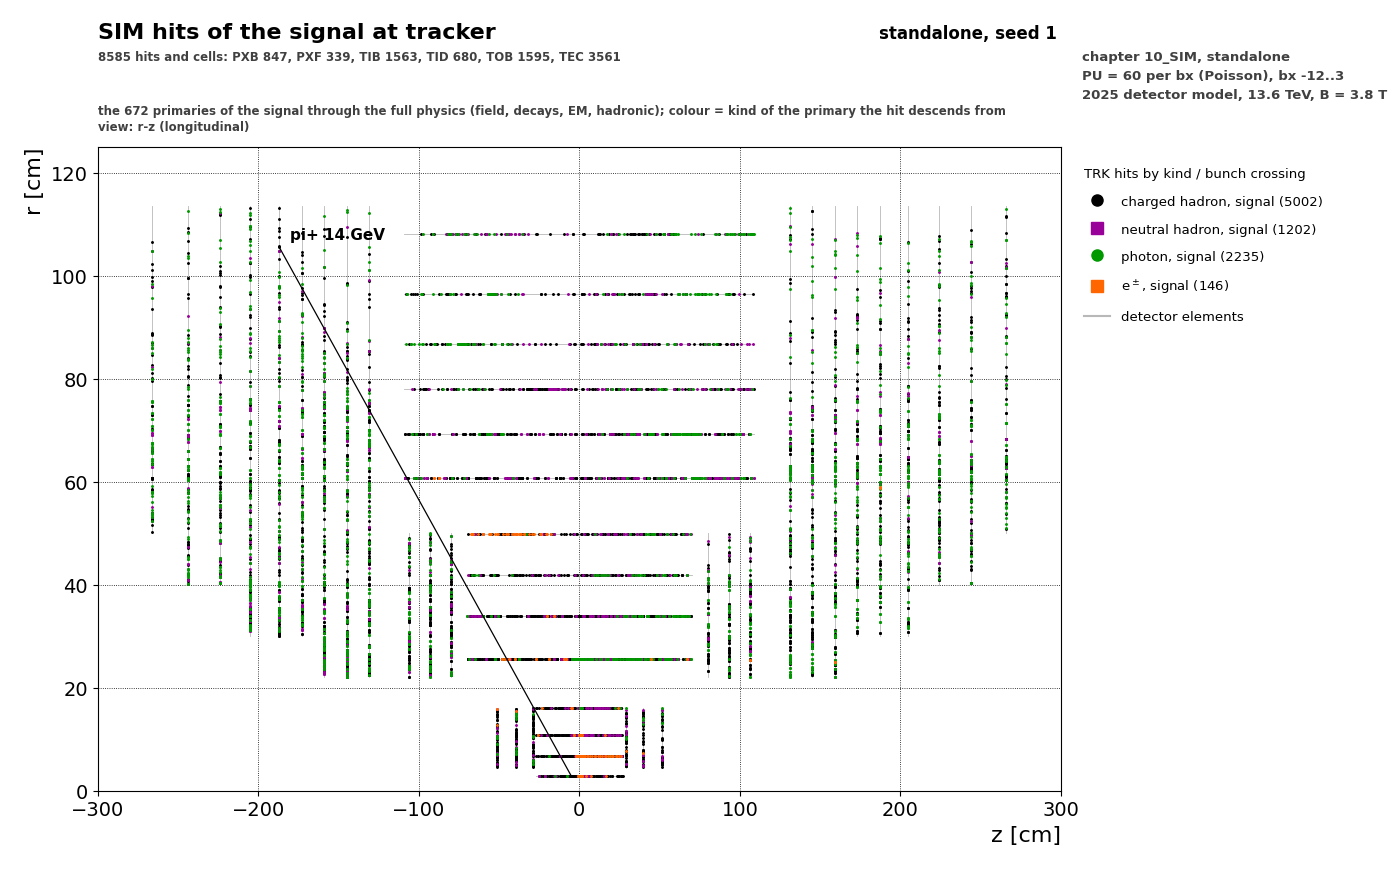
\includegraphics[width=0.495\textwidth]{SIM/Standalone/pages/simHits_signal_10_SIM_TRK_rz.png}\hfill
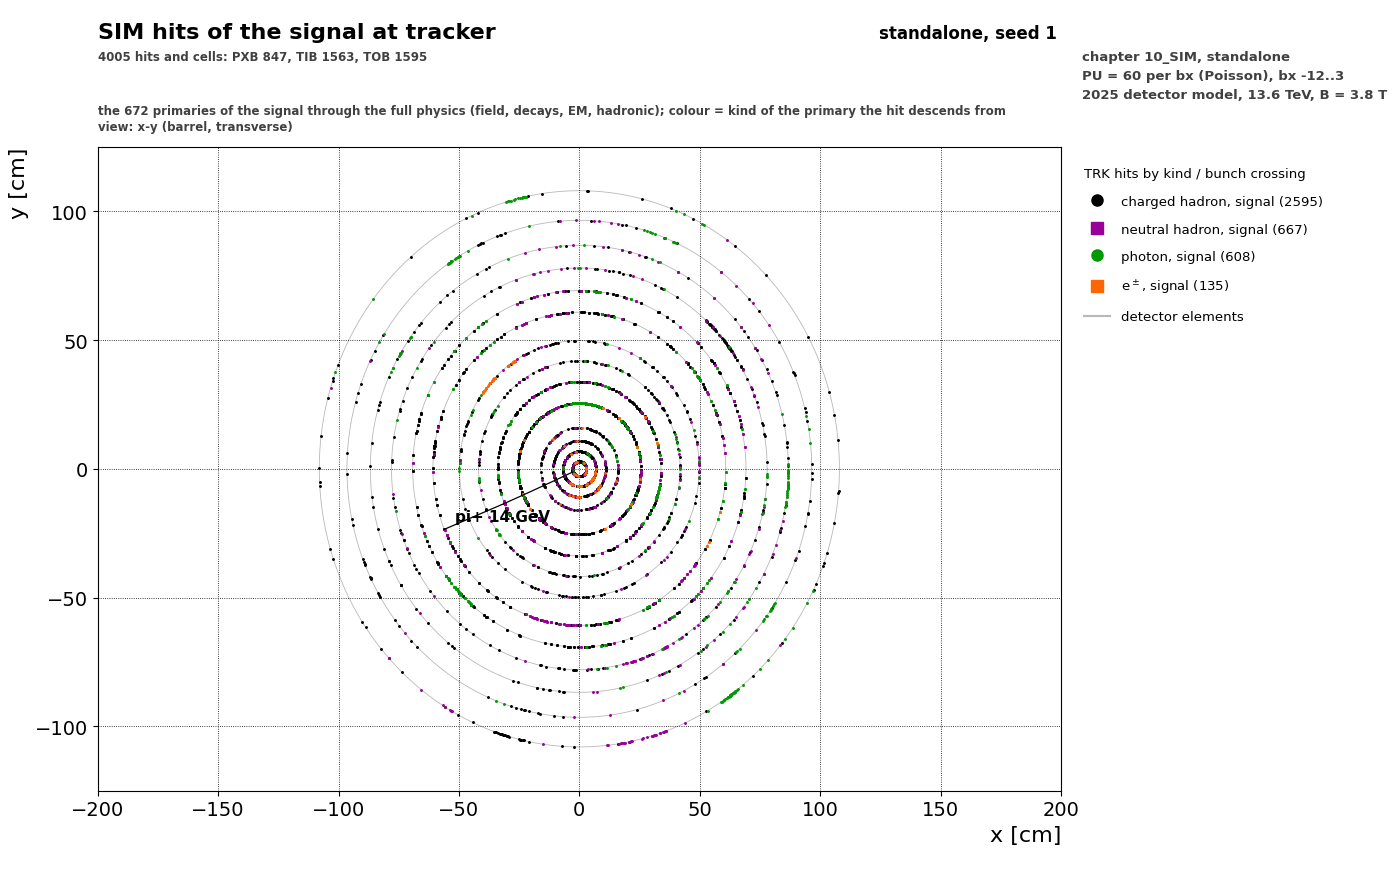
\includegraphics[width=0.495\textwidth]{SIM/Standalone/pages/simHits_signal_10_SIM_TRK_xy.png}\\[2pt]
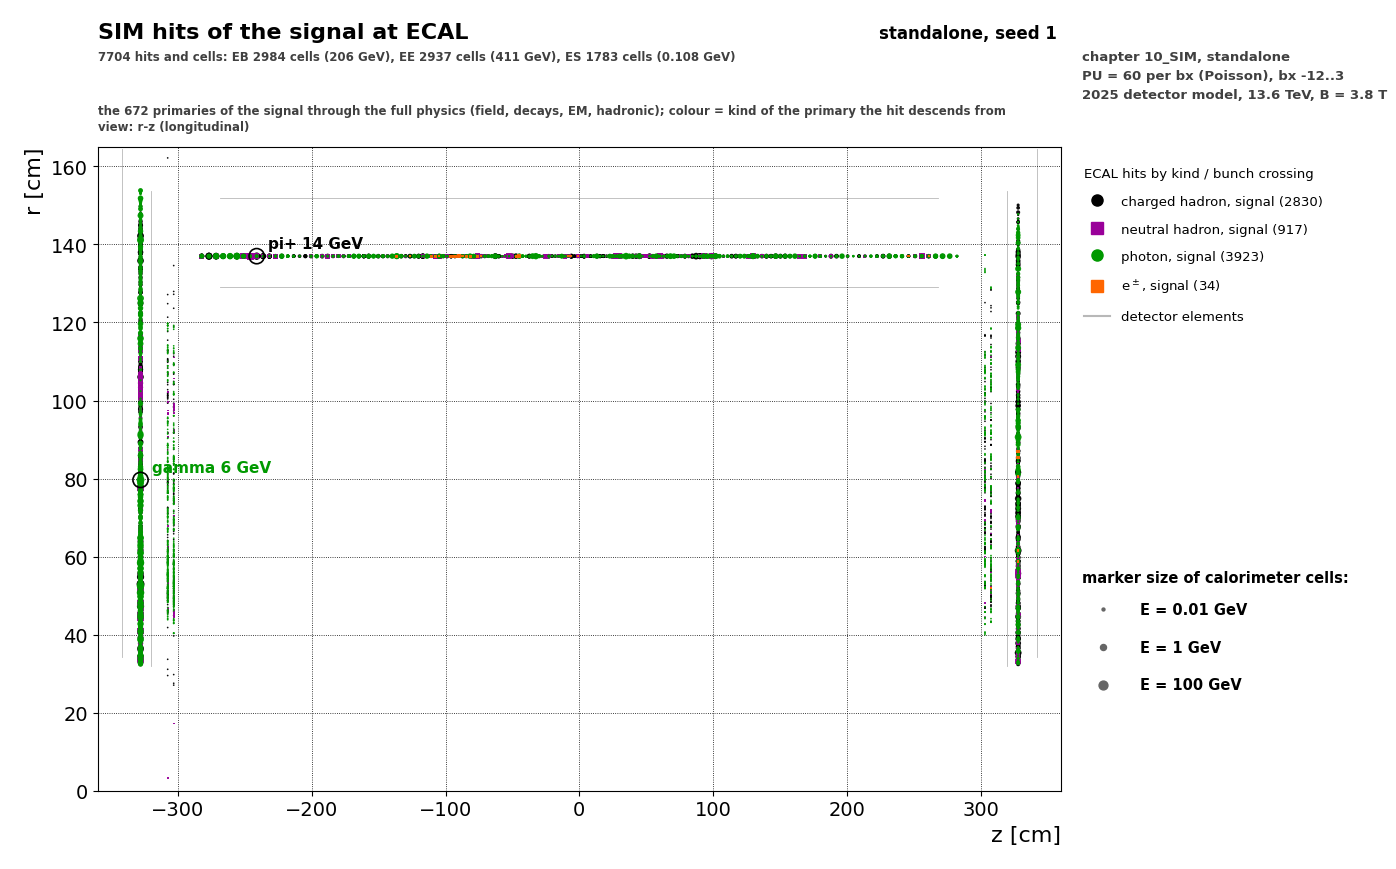
\includegraphics[width=0.495\textwidth]{SIM/Standalone/pages/simHits_signal_10_SIM_ECAL_rz.png}\hfill
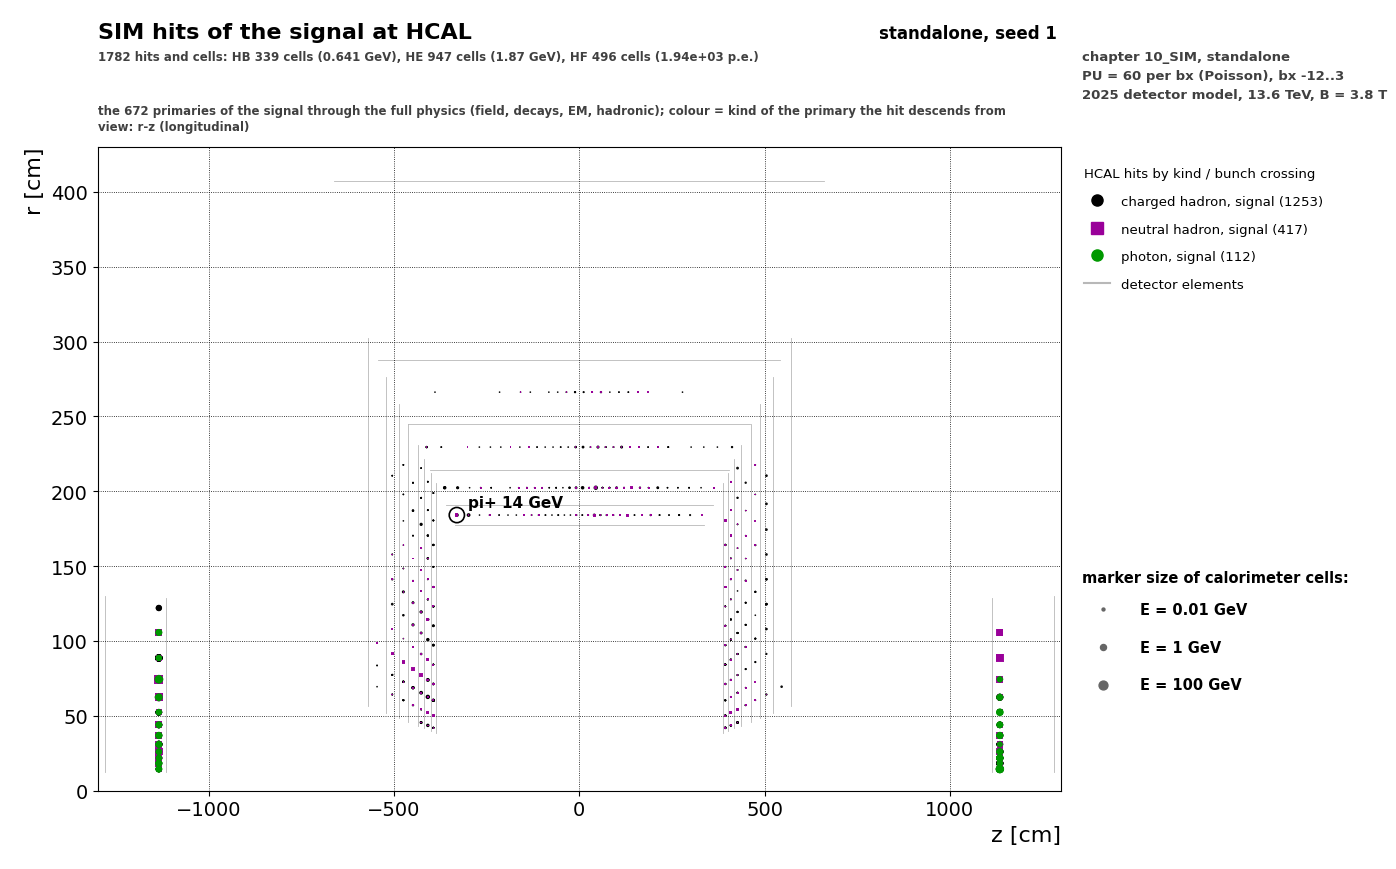
\includegraphics[width=0.495\textwidth]{SIM/Standalone/pages/simHits_signal_10_SIM_HCAL_rz.png}
\caption[The family station by station]{The family station by station
(\file{plot_simhits_SIM.py}). Top: the tracker in $r$--$z$ and its barrel in
$x$--$y$; bottom: ECAL and HCAL in $r$--$z$. A hit takes the colour of the
kind of primary it descends from: black charged hadrons, purple neutral
hadrons, green photons, orange electrons. The leading charged member of our
jet and the hardest photon are joined hit by hit.}
\label{fig:crowd_at_the_border:stations_signal}
\end{figure}

\begin{figure}[htbp]\centering
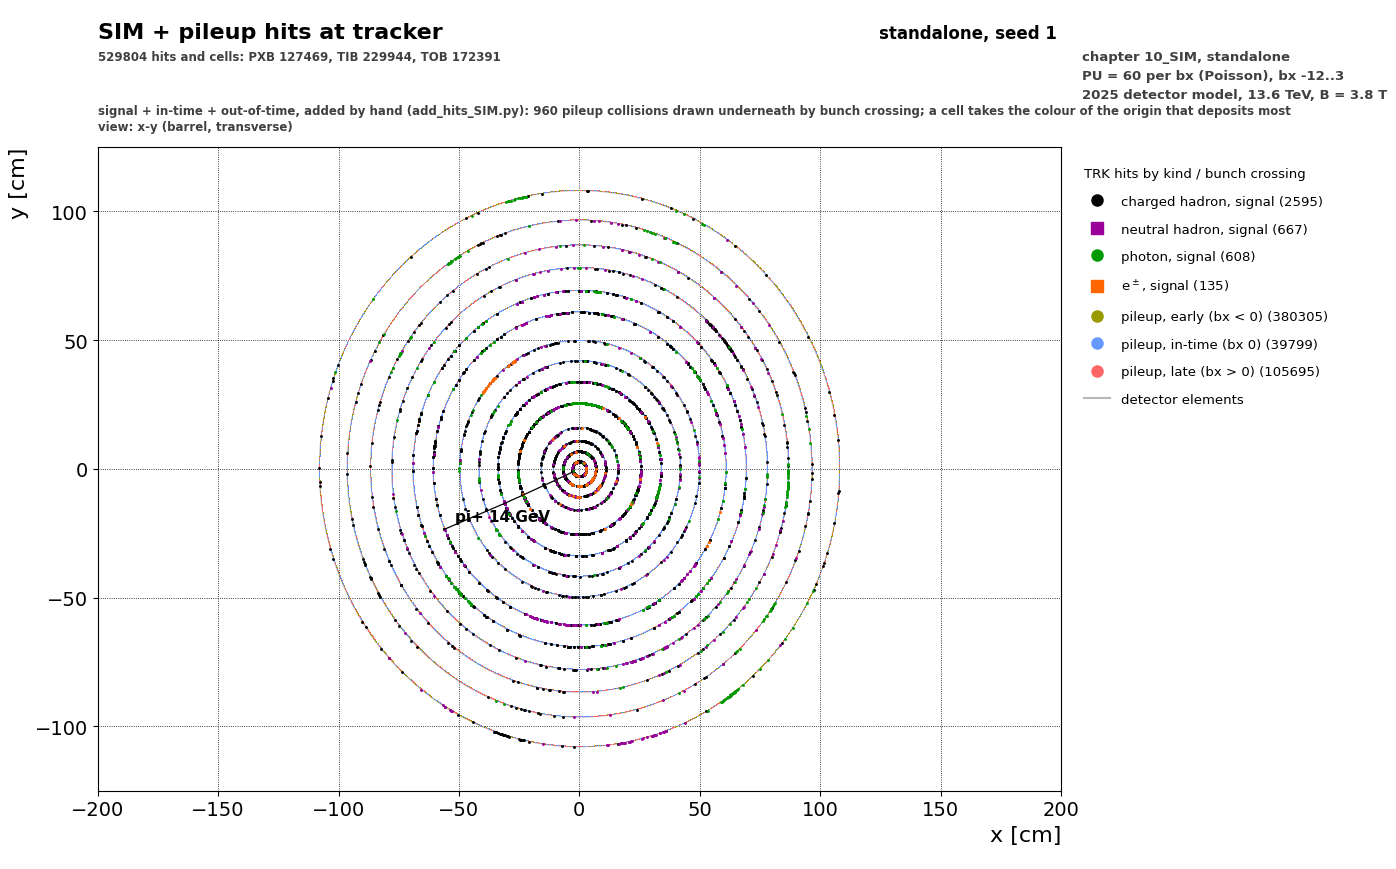
\includegraphics[width=0.495\textwidth]{SIM/Standalone/pages/simHits_mixed_10_SIM_TRK_xy.png}\hfill
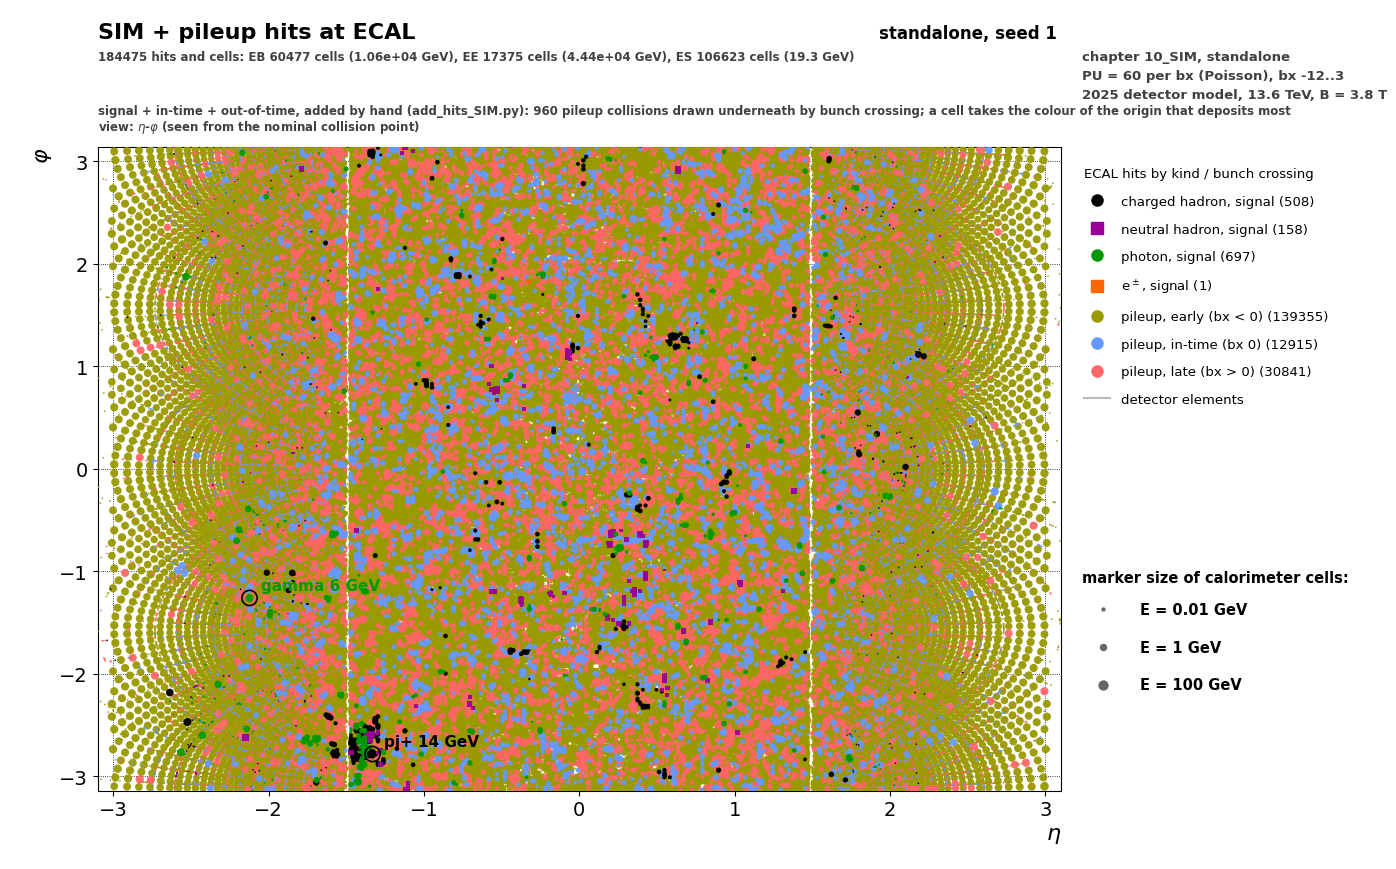
\includegraphics[width=0.495\textwidth]{SIM/Standalone/pages/simHits_mixed_10_SIM_ECAL_etaphi.png}\\[2pt]
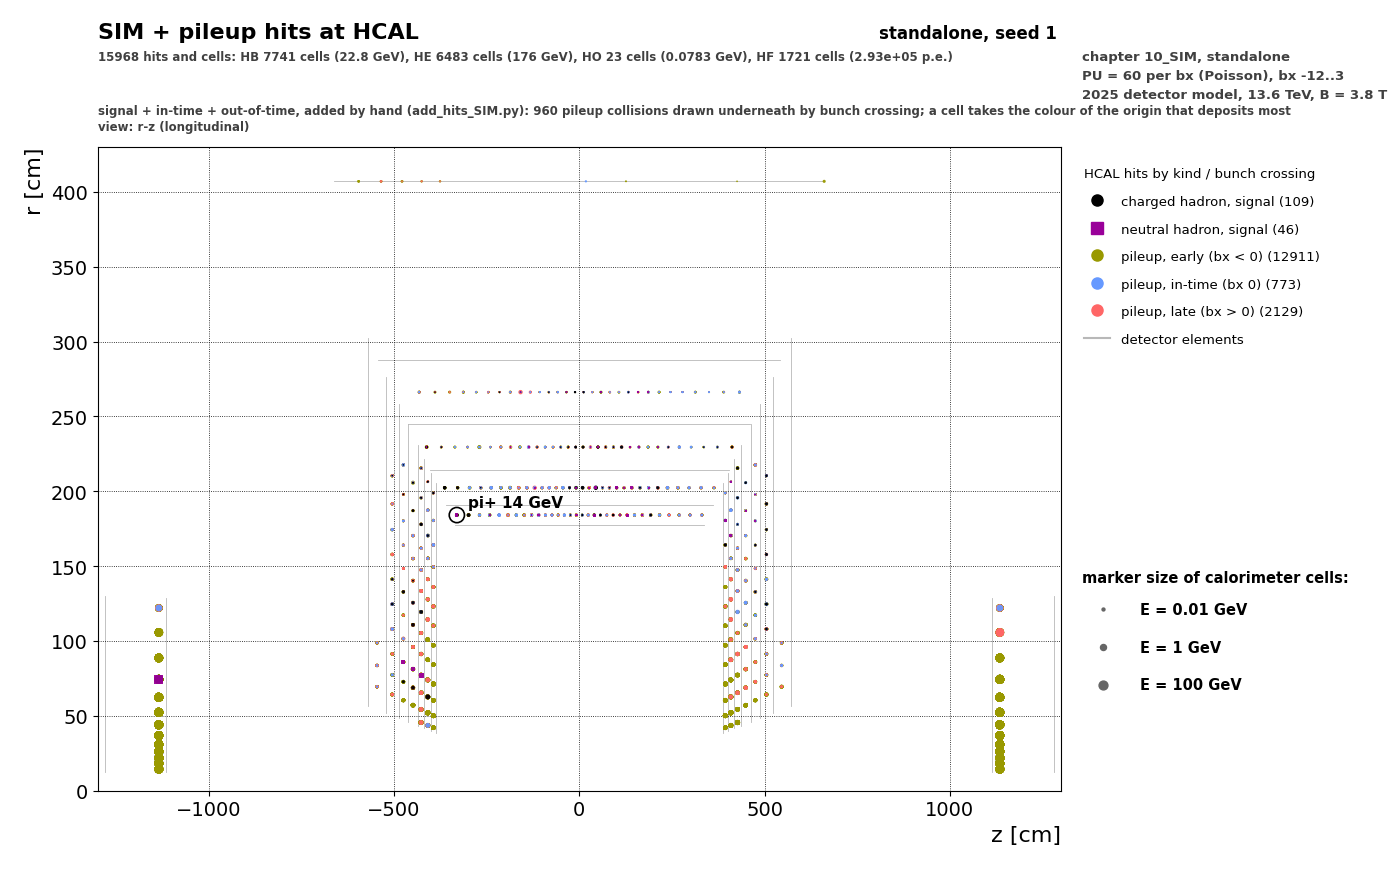
\includegraphics[width=0.495\textwidth]{SIM/Standalone/pages/simHits_mixed_10_SIM_HCAL_rz.png}\hfill
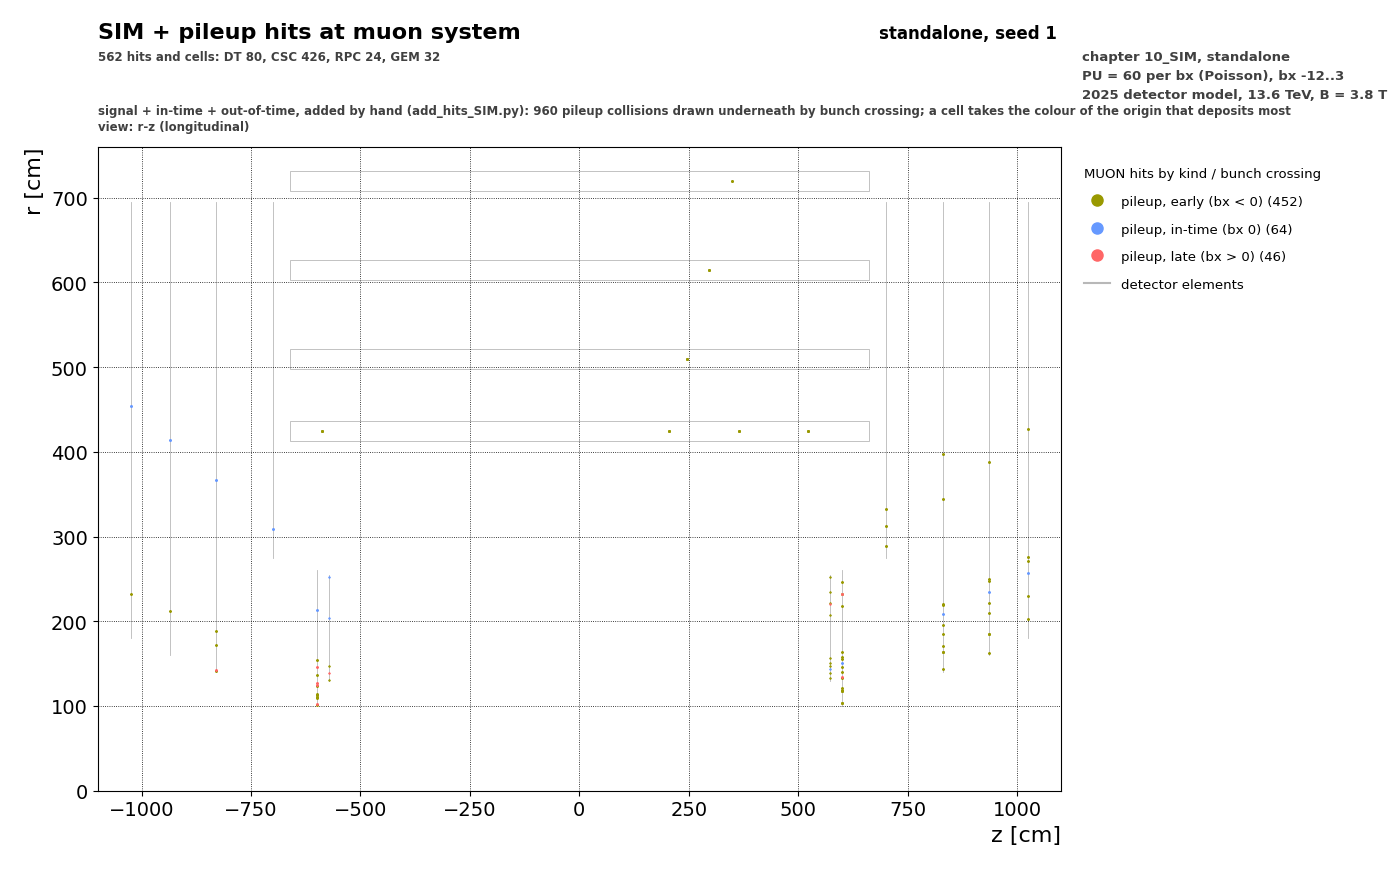
\includegraphics[width=0.495\textwidth]{SIM/Standalone/pages/simHits_mixed_10_SIM_MUON_rz.png}
\caption[The sum station by station]{The sum station by station: the
tracker barrel in $x$--$y$, the ECAL in $\eta$--$\phi$, the HCAL and the
muon system in $r$--$z$. The crowd is drawn underneath by bunch crossing,
olive early, blue in time, red late; a cell takes the colour of whoever
deposits most in it.}
\label{fig:crowd_at_the_border:stations_mixed}
\end{figure}

\paragraph{Our jet.}
\Cref{tab:crowd_at_the_border:ledger} follows the photograph of
\cref{ch:family_photograph} across the border. Its $31$ members carry
$222.8\GeV$ towards $\eta=-1.44$, the corner where the barrel meets the
endcap. Only $13$ of them reach the calorimeters as themselves, with
$44.3\GeV$ of vector \pt: ten photons converted, seven hadrons interacted in
the tracker, the $K^0_S$ decayed. Nothing is lost by that; the energy
arrives as secondaries. What is lost shows in the next row: the cells
record $133.5\GeV$ in $942$ crystals and $0.31\GeV$ in the scintillator of
$151$ HCAL cells, $46\GeV$ after the sampling factor, and their vector sum
is $73.5\GeV$ of the $99.8$. The difference is the physics of
\cref{sec:crowd_at_the_border:hadronic}: invisible energy, the response of
the calorimeters to hadrons, loopers that never arrive, and the gap between
barrel and endcap that this jet happens to point at.
\Cref{tab:crowd_at_the_border:circle} then counts everything the detector
receives inside the circle of the jet.

\begin{ledgerboth}{The Crossing of the Border}{tab:crowd_at_the_border:ledger}{From
the third row on, \pt is the vector sum of calorimeter cells seen from the
collision point, HCAL cells multiplied by the sampling factors of
\cref{ch:customs_form} ($125$ barrel, $190$ endcap), and
$n_{\mathrm{const}}$ counts cells. The \CMSSW rows follow its $b$ system, the
visible descendants of the $B^-$.}
\ledgerblock{Standalone (seed 1, \file{event_SIM.lhe})}
\ledgerrow{the photograph, \akfour jet [0], handed to \GEANT (chapter 9)}{99.83}{14.83}{31}{--}
\ledgerrow{its members reaching the calorimeters as primaries}{44.32}{--}{13}{$-55.51$}
\ledgerrow{what the cells record of its members and their secondaries}{73.52}{--}{1093}{$+29.20$}
\ledgerrow{all cells of the family in the circle $\Delta R<0.4$}{65.21}{--}{560}{$-8.31$}
\ledgerrow{\quad with the in-time crowd}{80.41}{--}{--}{$+15.20$}
\ledgerrow{\quad with the early crowd, $\bx=-12\ldots-1$}{247.03}{--}{--}{$+166.62$}
\ledgerrow{\quad with the late crowd, $\bx=+1\ldots+3$}{291.97}{--}{1655}{$+44.94$}
\ledgerblock{\CMSSW (run 1, event 1)}
\ledgerrow{the photograph, \akfour jet [0] (chapter 7)}{117.79}{16.72}{24}{--}
\ledgerrow{the $b$ system handed to \GEANT (chapter 9)}{56.82}{--}{8}{--}
\ledgerrow{its members reaching the calorimeters as primaries}{24.4}{--}{3}{$-32.4$}
\end{ledgerboth}

\begin{table}[htbp]\centering\footnotesize\setlength{\tabcolsep}{4pt}
\caption[The circle of our jet, by origin]{The circle of our jet,
$\Delta R<0.4$ around $(\eta,\phi)=(-1.44,-2.71)$: tracker hits, crystals
with energy, their energy and transverse energy, HCAL cells, the energy in
their scintillator and its transverse energy after the sampling factor, and
the sum of the two transverse energies, in GeV.}
\label{tab:crowd_at_the_border:circle}
\begin{tabular}{@{}lrrrrrrrr@{}}\toprule
 & tracker & \multicolumn{3}{c}{crystals} & \multicolumn{3}{c}{HCAL} & $\sum E_T$ \\
 & hits & cells & $E$ & $E_T$ & cells & $E_{\mathrm{scint}}$ & $E_T\times$factor & \\ \midrule
\simCircleRows
\bottomrule
\end{tabular}
\end{table}

\paragraph{The same event in \CMSSW.}
\label{sec:crowd_at_the_border:cmssw_event}
The companion runs \GEANT itself, four times on the signal with one
ingredient more each time, once on a library of $1000$ minimum-bias
collisions, and then the \Mix without its digitisers on $995$ of them.
Its stage table reads like ours: the primaries reaching the boundary fall
from $557$ to $310$ of $571$, the secondaries grow to $1355$, the tracker
hits from $6734$ to $10\,272$ with $2.33\GeV$ of energy loss, and the muon
chambers fill with $522$ hits when hadrons can ionise but not interact. Its
$b$ system, eight primaries with $140.3\GeV$ pointing at the endcap, reaches
the boundary with three of them and $24.4\GeV$ of \pt, and leaves
$63.6\GeV$ in the crystals and $0.39\GeV$ in the scintillator, about
$73\GeV$ after the sampling factor: half in each calorimeter, as for our
jet. One of its photons, $44\GeV$, is the lesson of
\cref{fig:crowd_at_the_border:shower} in a single particle: unconverted in
one run, it puts two thirds of its energy in one crystal; converted in the
first pixel layer in another, it lights $466$. In the sum the signal is
$0.49\,\%$ of $2.1$ million tracker hits and keeps $699$ of its $12\,804$
ECAL cells. The displays of \cref{fig:crowd_at_the_border:displays} are the
two events at this stage.

\begin{figure}[p]\centering
\ledgerdisplays
  {SIM/Standalone/pages/simHits_mixed_10_SIM_ALL_etaphi.png}
  {Standalone: the family with the $960$ collisions of its crowd underneath (\file{plot_simhits_SIM.py}).}
  {fig:crowd_at_the_border:journey}
  {SIM/CMSSW/simHits_mixed_10_SIM_ALL_etaphi_run1_event1.png}
  {\CMSSW: the signal with its $995$ pileup collisions, the \code{SimHitAnalyzer} page of \code{JitJetSW}.}
  {fig:crowd_at_the_border:cmssw}
\caption[The simulated hits in the $(\eta,\phi)$ plane, standalone and
\CMSSW]{Every simulated hit and cell in the $(\eta,\phi)$ plane, standalone
(a) and \CMSSW (b): the family by kind of primary, the crowd by bunch
crossing (olive early, blue in time, red late), cells sized by energy. In
both the family survives as the strings of its charged tracks and the cores
of its jets, ours at $(-1.4,-2.7)$ in (a).}
\label{fig:crowd_at_the_border:displays}
\end{figure}

\subsection{What this stop is, and what it is not}
\label{sec:crowd_at_the_border:caveats}
\begin{itemize}
  \item \textbf{A simulation in the spirit of \GEANT, not \GEANT.} The
    detector is $54$ surfaces and seven kinds of cells; a shower is a
    parametrised cloud of spots, a nuclear interaction in the tracker a toy
    model of pions and nucleons. The material is tuned to the CMS geometry;
    the calorimeter constants ($h/e$, the sampling fractions, the
    photoelectrons per \GeV of the HF) are chosen to give the scale of
    test beams and of the companion, not derived.
  \item \textbf{Fewer soft hits than \GEANT.} The script creates no
    $\delta$ rays, no Compton electrons and no nuclear fragments, and stops
    a particle below $10\MeV$. It has $12.8$ tracker hits per primary where
    \GEANT has $18.0$, and counts as hit only cells that received a spot of
    a few \MeV, where \GEANT keeps every deposit above $15\keV$. Cell
    counts of the two are not comparable; energies are.
  \item \textbf{The field is a box.} $3.8$~T inside $|z|<6.5$~m and nothing
    outside; the return field in the yoke, which bends muons back, is not
    there, and a muon flies straight from the HCAL to its stations.
  \item \textbf{SimHits are energy, not signals.} No pulse shape, no noise,
    no threshold, no time window: all sixteen crossings are in the sum with
    equal weight. The $231\GeV$ of the crowd in our circle is what the
    detector receives, not what it will read out.
  \item \textbf{One event is one sample}, and the two events of the stop are
    different events.
\end{itemize}

\section{Further reading}
\label{sec:crowd_at_the_border:further_reading}
The physics of this stop is the review of the passage of particles through
matter of the Particle Data Group~\cite{ParticleDataGroup:2024cfk}, and for
calorimeters the book of Wigmans~\cite{Wigmans:2000vf} and the review of
Fabjan and Gianotti~\cite{Fabjan:2003aq}. The detector is described
in~\cite{CMS:2008xjf,CMS:2024aqx}, its tracker material as measured with
nuclear interactions in~\cite{CMS:2018wqs}, the response of its barrel
calorimeters to hadrons in~\cite{USCMS:2009fxn}. The simulation of CMS with
\GEANT, its physics list and its validation are
in~\cite{CMS:2021dly,Srimanobhas:2024nmy,Banerjee:2017bhj}, the models
behind the list in~\cite{Wright:2015xia}, the fast simulation
in~\cite{Abdullin:2011zz,Rahmat:2011xp}, the mixing and premixing
in~\cite{Hildreth:2017caz}.

\begin{pitfalls}
\begin{itemize}[nosep]
  \item \emph{``A particle below $0.7\GeV$ leaves no energy in the
    calorimeter.''} It leaves none in the barrel. It spirals to the endcap
    and arrives there, late and far from where it was aimed.
  \item \emph{``The primaries at the boundary fell from $672$ to $407$, so a
    third of the energy is lost.''} The count is of particles that arrive
    as themselves. A converted photon arrives as two electrons with all of
    its energy.
  \item \emph{``The HCAL holds $2.5\GeV$, so the hadrons deposit almost
    nothing.''} A SimHit of a sampling calorimeter is the energy in the
    scintillator, about $1\,\%$ of what the calorimeter absorbed. And an HF
    hit is not an energy at all but a number of photoelectrons.
  \item \emph{Radiation length and interaction length are different units.}
    The crystals are $26\,\Xzero$ but $1.1\,\lamI$ deep: a wall for a
    photon, a window for one pion in three.
  \item \emph{Is the signal simulated together with its pileup?} Never. They
    meet at the level of hits here, and in the production one step later,
    as digitised signals (premixing).
  \item \emph{``Out-of-time pileup is out of the event.''} At this stop it
    is three quarters of the event. The electronics decide how much of it
    stays.
\end{itemize}
\end{pitfalls}

\begin{exercises}
\item From \cref{eq:crowd_at_the_border:looper}: what field would let a
  pion of $0.3\GeV$ reach the barrel ECAL? Run
  \code{standalone\_SIM.py --sample signal --field 2 -v} and compare the
  loopers and the tracker hits with the $3.8$~T run.
\item Run the family with \code{--stage B\_Decay\_EM} and explain the $955$
  muon-chamber hits. Which hadrons make them, and why are they gone in the
  full simulation?
\item From the primary listing of \file{event_SIM.lhe}, take the photons
  above $1\GeV$ in $|\eta|<1$ and in $1.5<|\eta|<2.5$ and count the
  conversions. Deduce the material in each region with
  \cref{eq:crowd_at_the_border:conversion} and compare with
  \cref{fig:crowd_at_the_border:material}.
\item With \cref{eq:crowd_at_the_border:fem}, compute the response
  $f_{em}+(1-f_{em})h/e$ for one pion of $100\GeV$ and for ten pions of
  $10\GeV$. Which jet looks more energetic to the calorimeter?
\item In \file{add_hits_SIM.py}, set the shift to zero and compare the time
  distribution of the tracker hits with \cref{fig:crowd_at_the_border:time}.
  Then keep only the crossings $\bx=-3\ldots+3$, the Phase-2 window of the
  release, and recompute the circle of our jet.
\item For the HL-LHC, scale the in-time column of
  \cref{tab:crowd_at_the_border:hits_ledger} to $200$ collisions. How many
  tracker hits per crossing, and what share is the family's?
\end{exercises}

\subsection*{Open problems in the context of Phase-2 LHC}
\label{sec:crowd_at_the_border:open_problems}
\begin{enumerate}
  \item \textbf{The CPU budget of full simulation.} The move to Run~3 gained
    about $25\,\%$ in speed~\cite{CMS:2021dly}; the plan for Phase-2 is, in
    the words of the collaboration, very ambitious~\cite{Srimanobhas:2024nmy,Srimanobhas:2025abv},
    and the community asks for large factors~\cite{HEPSoftwareFoundation:2018fmg,Apostolakis:2022nnf}
    within a computing model that is itself being
    revised~\cite{Perez-CaleroYzquierdo:2026dvu}. Our crowd costs $140$ times
    the family at $60$ collisions and sixteen crossings; at $200$ the ratio
    more than triples.
  \item \textbf{A calorimeter of six million channels.} The HGCAL~\cite{CMS:2017jpq}
    replaces the endcap crystals and tiles of this chapter by silicon pads
    and small tiles in $47$ layers. Its prototypes agree with \GEANT for
    positrons and pions of $20$ to $300\GeV$~\cite{CMSHGCAL:2021nyx,CMS:2022jvd},
    the first such test of hadronic showers at this granularity; whether the
    physics list describes the substructure of a shower, and at what cost
    per event, is open.
  \item \textbf{Time as a fourth coordinate.} The timing layer~\cite{Butler:2019rpu}
    aims at $30$ to $40$~ps per track and needs hit times simulated to that
    precision~\cite{Sorrentino:2023hjw}. The time structure of a hadronic
    shower depends on its slow neutrons~\cite{CALICE:2014tgv}, the part of
    the physics that fast physics lists cut first, and that this chapter
    called invisible.
  \item \textbf{The hadronic models and the jet energy scale.} Single-hadron
    response in data and \GEANT differs by up to $5\,\%$, which becomes a
    jet-scale uncertainty of $2$ to $5\,\%$ for the hardest
    jets~\cite{ATLAS:2016djy}. Tunes of the hadronic models with
    uncertainties are only beginning~\cite{Genser:2023fic}; no uncertainty
    model exists for a new calorimeter before it takes data.
  \item \textbf{Transport on graphics processors.} Electromagnetic
    transport runs $6$ to $32$ times faster on a GPU, but a full application
    with hadronic physics gains only a factor of about
    two~\cite{Johnson:2024qqt}, and the first integrations into experiment
    frameworks met difficulties~\cite{Apostolakis:2025vca}; the options of
    \GEANT~11 for faster electromagnetic physics are being
    adopted~\cite{Hahnfeld:2024zrb}.
  \item \textbf{Learning the simulation.} Machine-learned refinement of the
    fast simulation~\cite{Bein:2023ylt}, generative calorimeter
    showers~\cite{Amram:2023onf,Krause:2024avx} and end-to-end models that
    skip the hits altogether~\cite{Vaselli:2024vrx,Vaselli:2025fov} are
    orders of magnitude faster. How to validate them, and what systematic
    uncertainty to assign to a jet they produced, is unsolved; and a model
    that skips the hits cannot answer the question of this chapter, whose
    hit it was.
  \item \textbf{The premixed crowd at 200.} The production digitises the
    crowd once and reuses it~\cite{Hildreth:2017caz}. The release mixes
    seven crossings of $200$ for Phase-2, $1400$ collisions per event; how
    large the premixed library must be, and what its reuse does to
    correlations between events, has not been quantified in a publication we
    could find.
\end{enumerate}
The family has crossed, and so has everyone else. The next stop turns what
the country received into numbers on a form.
